\section{知识表示与推理}
\subsection{逻辑Agent}
\subsubsection{基于知识的Agent}

\begin{figure}[htbp]
    \centering
    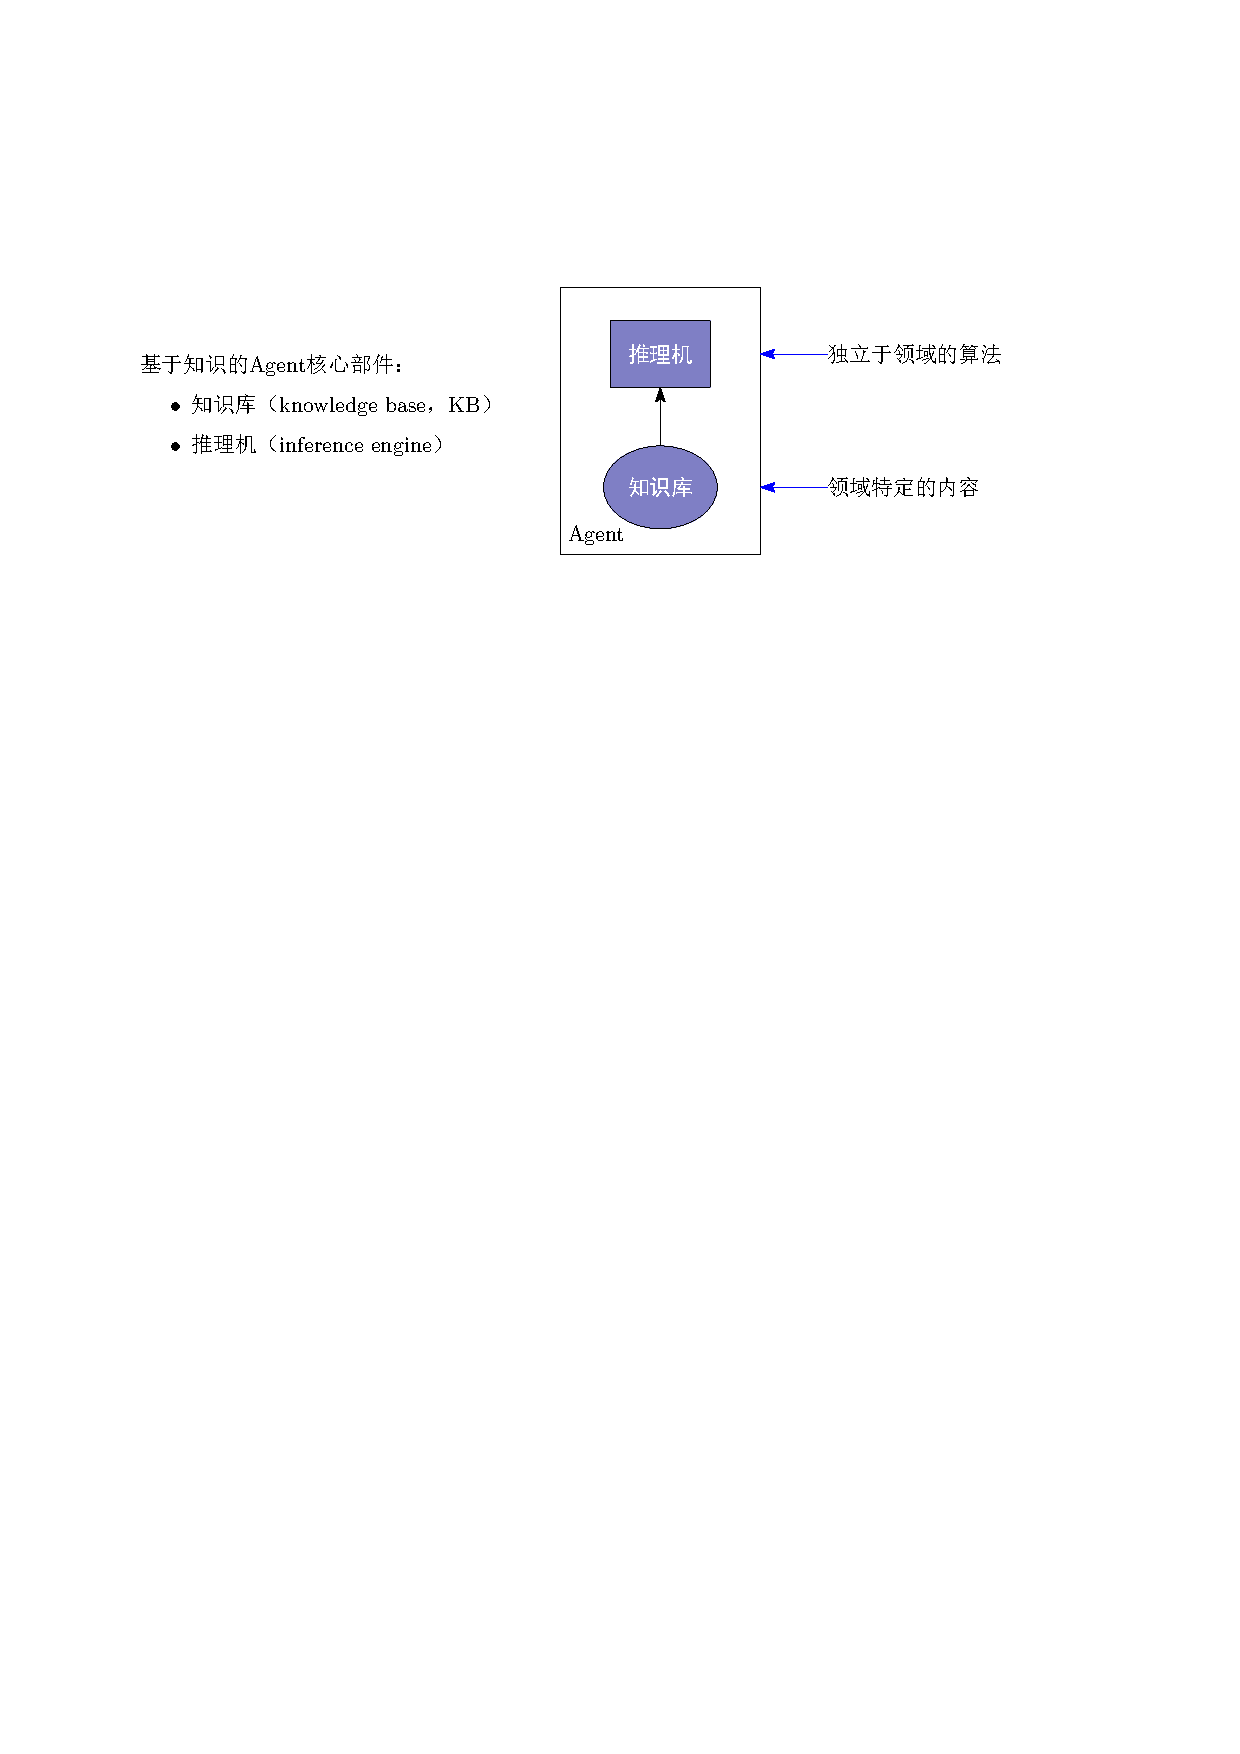
\includegraphics{image/基于知识的Agent.pdf}
\end{figure}

\begin{definition}[蕴含(Entailment)]
    知识库KB(一组对已知世界和规则描述的逻辑语句)蕴含语句$\alpha$(某个待确定的逻辑结论),当且仅当在KB为真的所有世界中$\alpha$也为真。蕴含表示为
    \[
        \textcolor{main1}{KB}\models\alpha 
    \]
    即,若$\textcolor{main1}{KB}\models\alpha $,当且仅当$M(KB)\subseteq M(\alpha)$
\end{definition}
\subsubsection{命题逻辑的推理}
\begin{figure}[htbp]
    \centering
    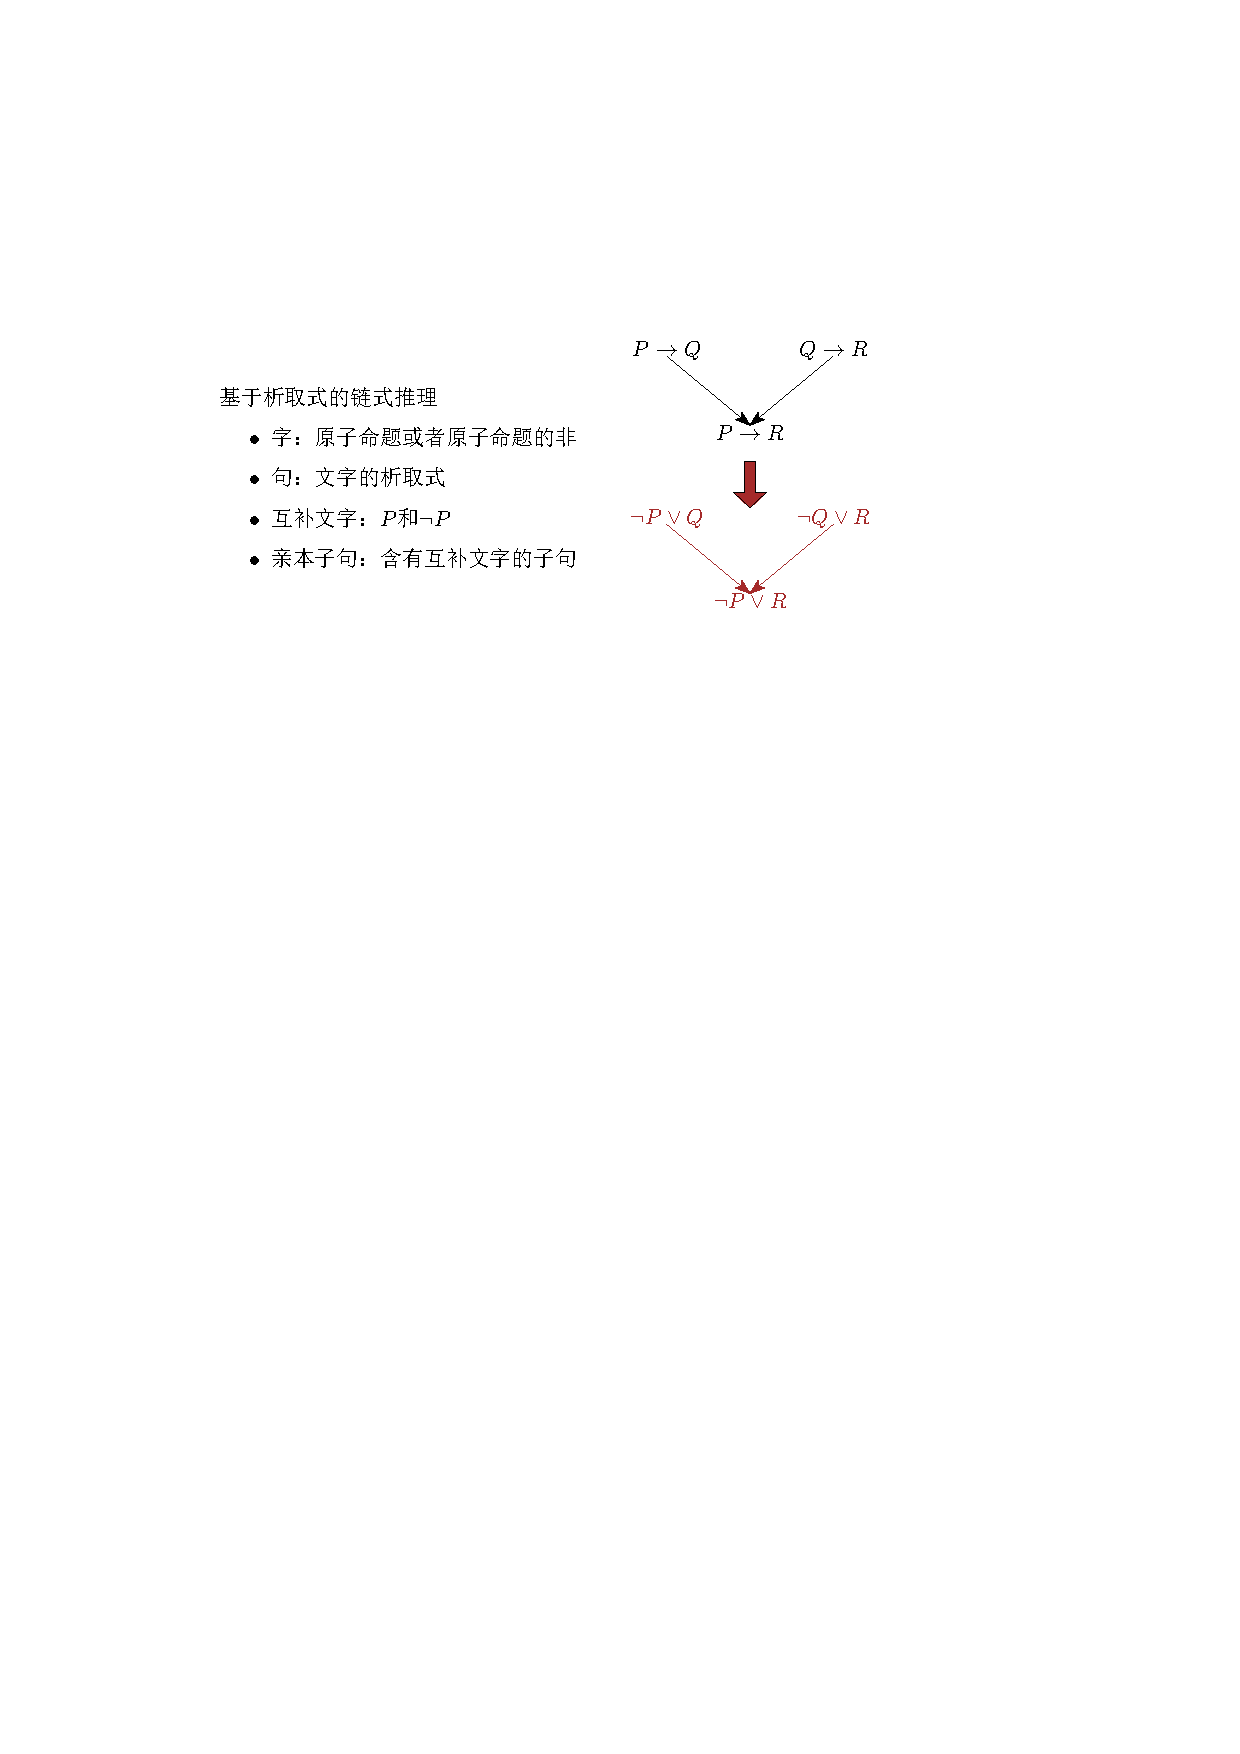
\includegraphics{image/基于析取式的链式推理.pdf}
\end{figure}
\begin{note}
    归结(Resolution):

    链式推理和假言推理都可以转化成相同的推理规则:\textcolor{main1}{两个含有互补文字的亲本子句可以进行推理,推理得到的结论是去除互补文字后两个子句的析取式。}
\end{note}
\begin{definition}[析取范式]
    设$A$为如下形式的命题公式$B_1\lor B_2\lor \dots\lor B_n$,其中$B_i,\ (i = 1,2,\dots, n)$为原子命题或其否定,则$A$称为析取范式或析取式。
\end{definition}
\begin{note}
    归结中需要注意的问题1:
    \begin{itemize}
        \item 进行归结之前,需要把已知的事实、定理等化成\textcolor{main1}{析取范式或者是单个文字的形式,}单个文字是原子命题,也可以看成一个析取范式。
        \item \textcolor{main1}{析取范式之间的逻辑关系是合取},也就是“与”因为子句表示的是已知事实或者定理,这些子句必须同时成立才能推导出结论。
    \end{itemize}
    子句间是合取关系,子句内是析取形式。
\end{note}
\begin{example}
    选取两个含有互补文字的子句进行归结,产生新的子句,如果新子句和原始子句含有互补文字,那么继续归结,直到再没有亲本子句。
    \begin{figure}[htbp]
        \centering
        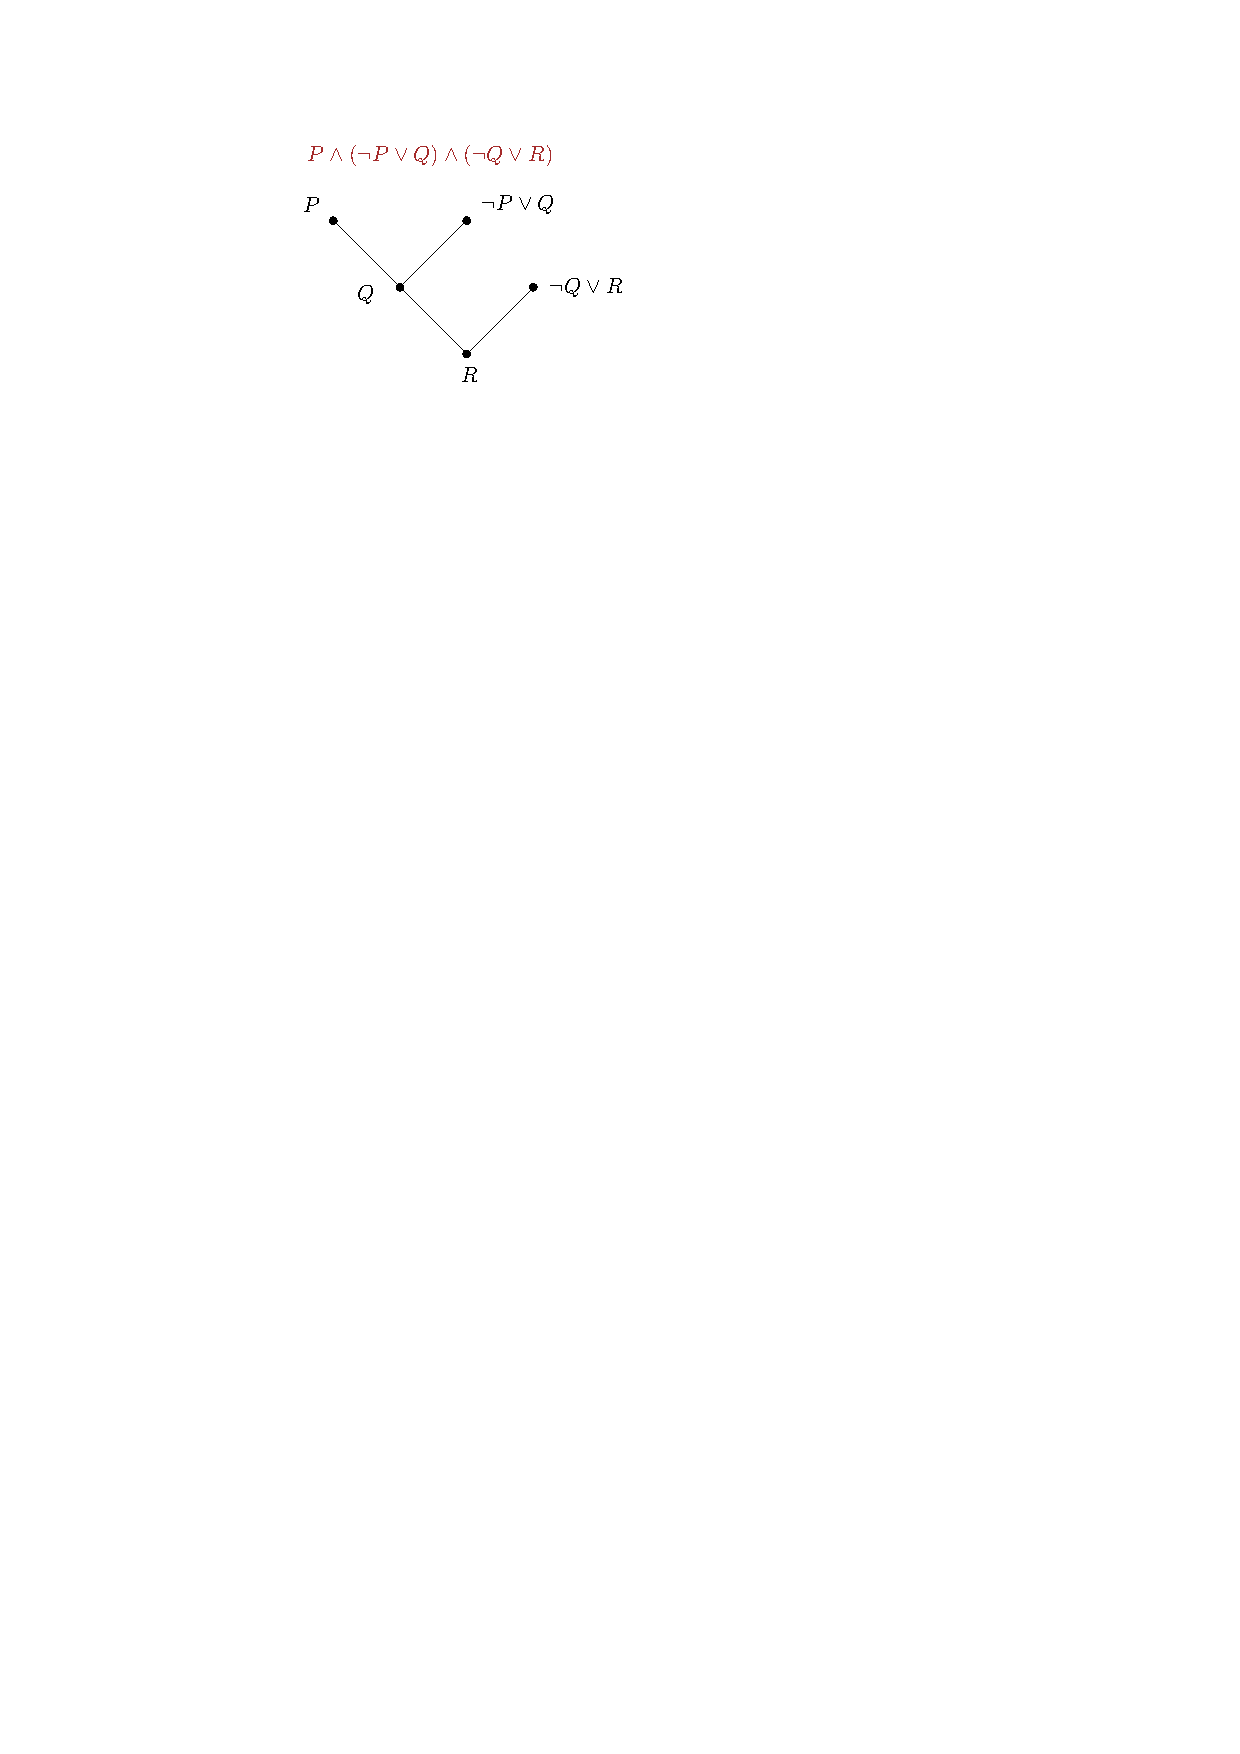
\includegraphics{image/归结.pdf}
    \end{figure}
\end{example}
\begin{example}
    将以下问题进行归结:
    \begin{enumerate}
        \item 将$\lnot P\lor Q\lor W$与$P\lor Q\lor R\lor S$归结。
        \begin{figure}[htbp]
            \centering
            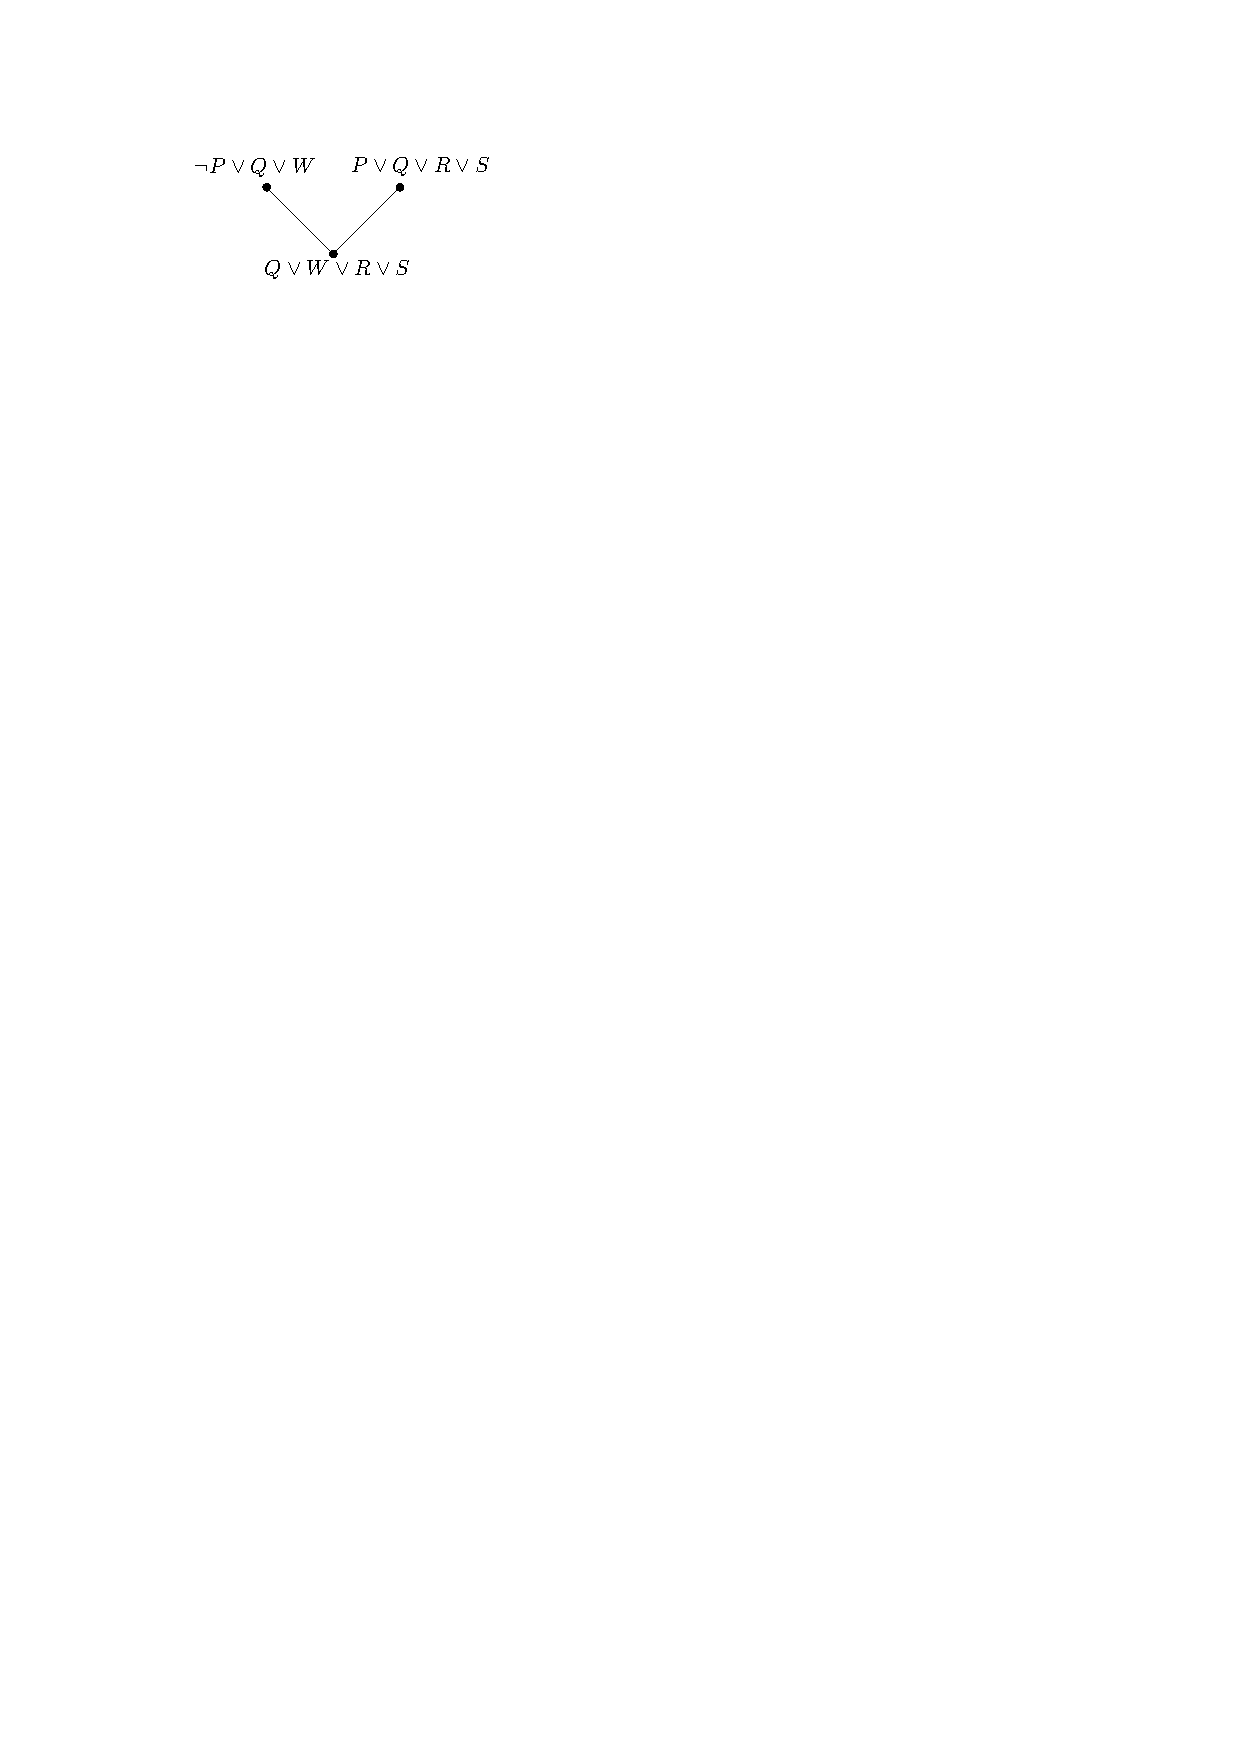
\includegraphics{image/归结-1.pdf}
        \end{figure}
        \item $P\lor W\lor \lnot Q\lor R$与$P\lor Q\lor \lnot R$归结的结果是什么?
        \begin{figure}[htbp]
            \centering
            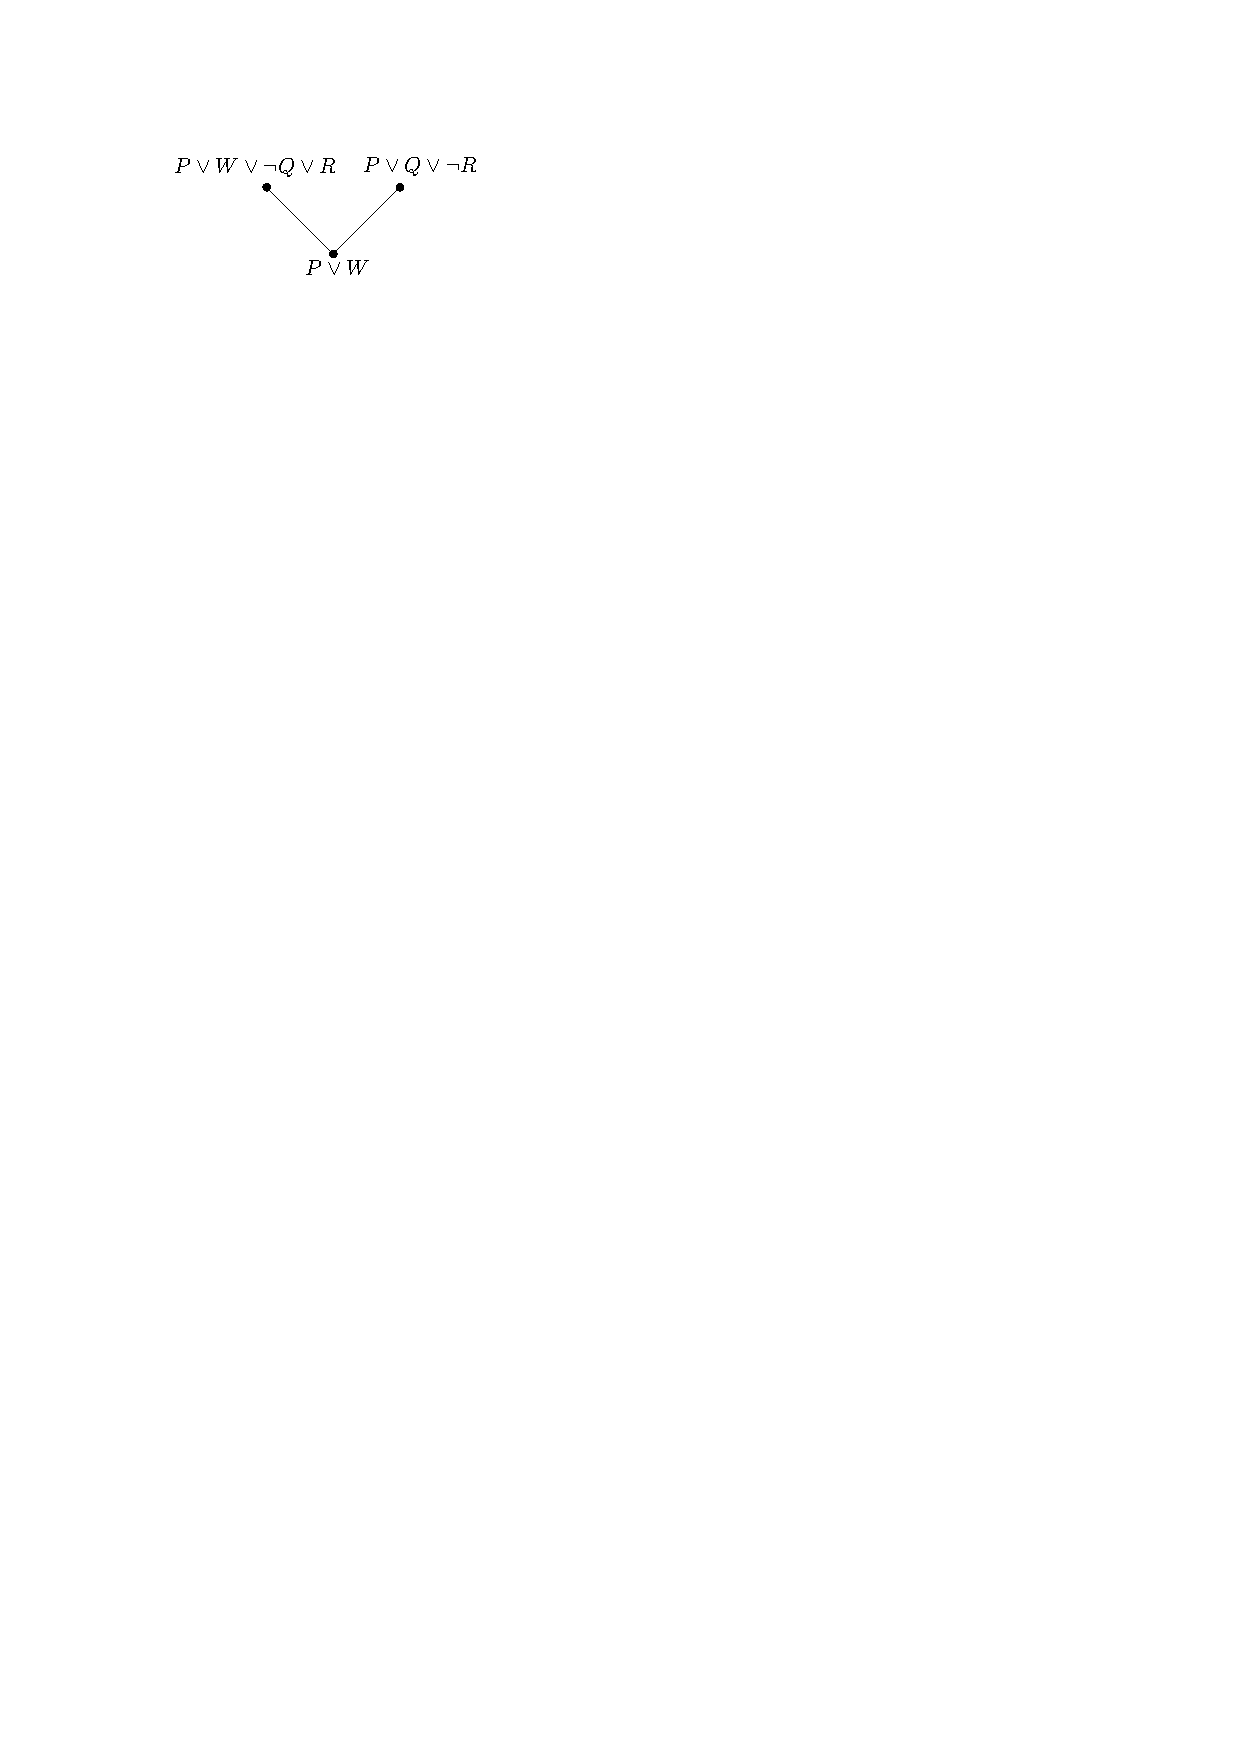
\includegraphics{image/归结-2.pdf}
        \end{figure}
        \item 将$P\lor \lnot Q$与$P\lor Q$以及$\lnot P$归结
        \begin{figure}[!h]
            \centering
            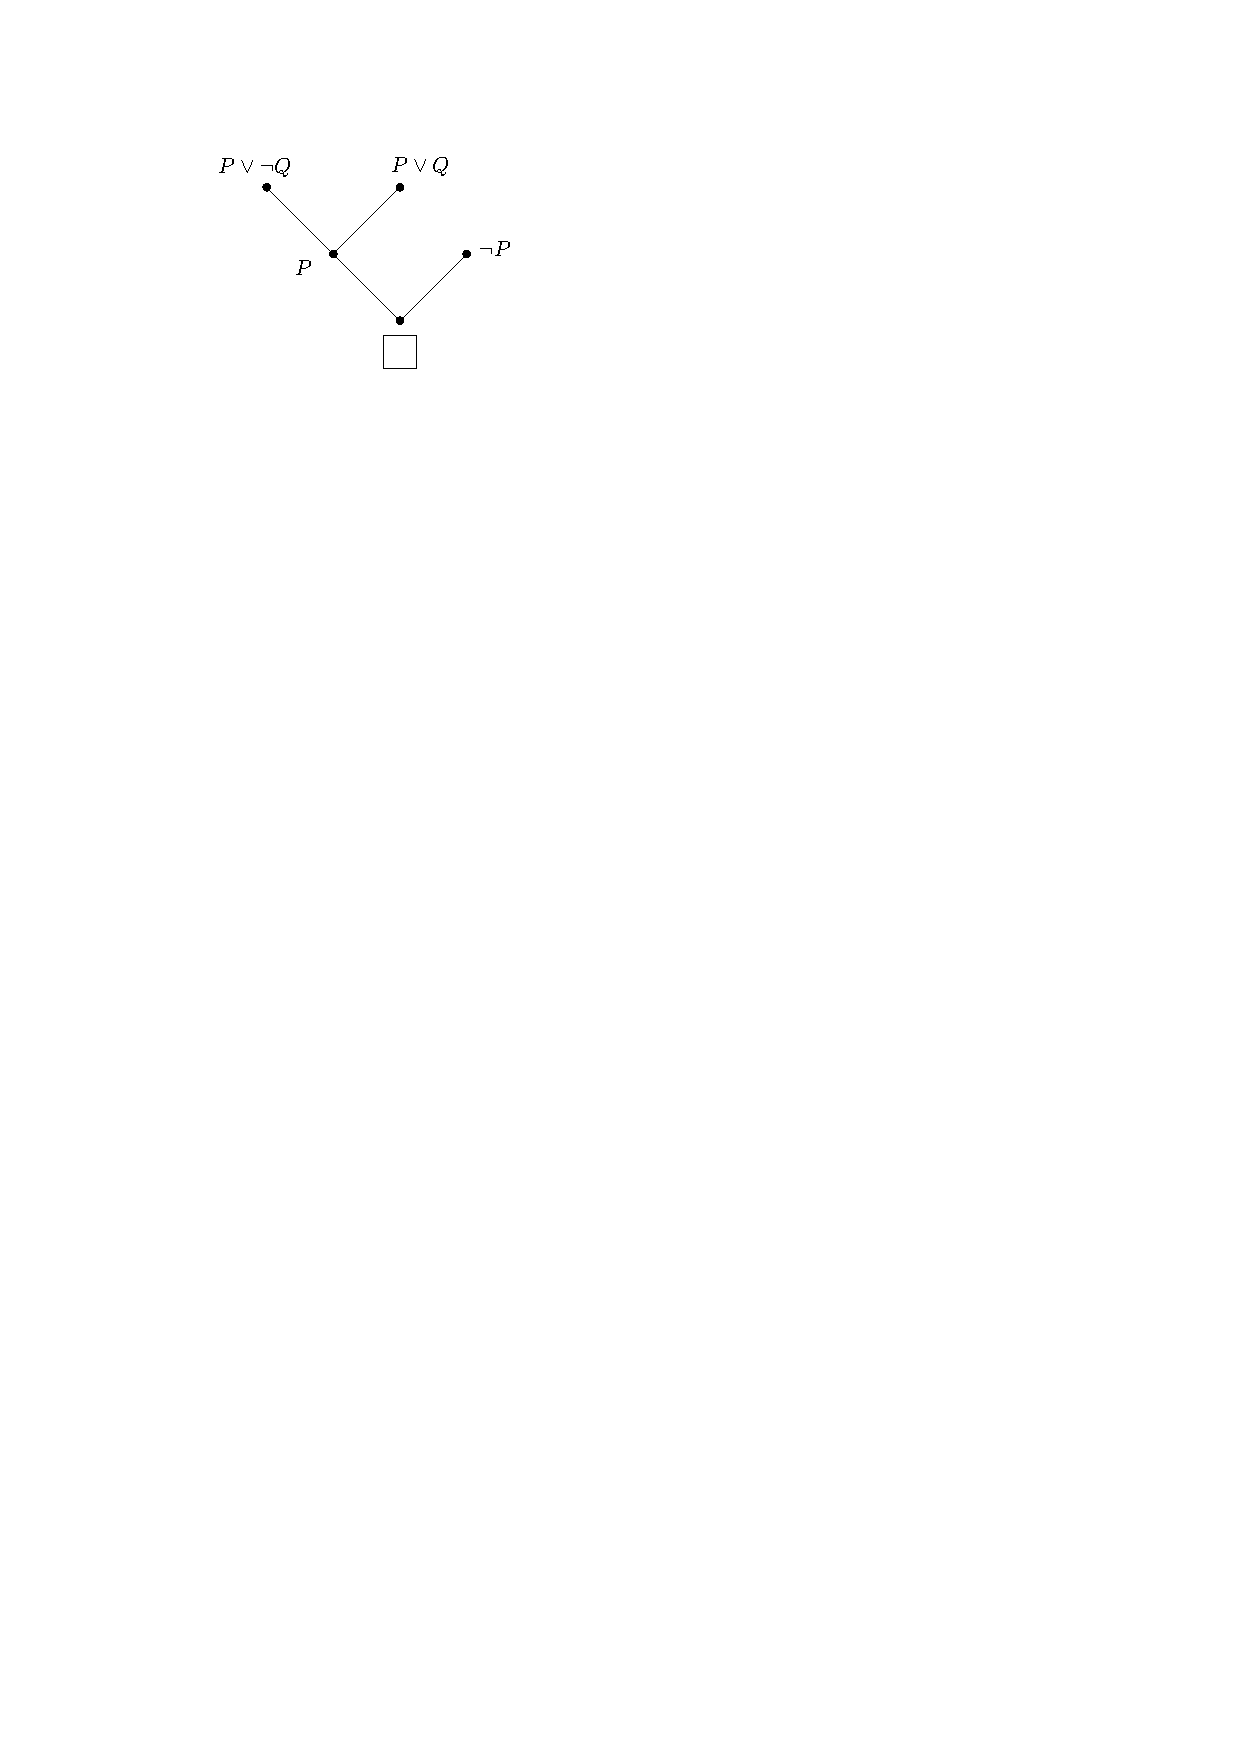
\includegraphics{image/归结-3.pdf}
        \end{figure}
    \end{enumerate}
\end{example}
\begin{definition}[空子句]
    不含任何文字的子句称为空子句。
    
    由于空子句不含有任何文字,也就不能被任何解释所满足因此空子句是永假的,不可满足的。
\end{definition}
\begin{note}
    归结中需要注意的问题2
    \begin{itemize}
        \item \textcolor{main1}{归结结果为空子句}意味着推导出的结果为\textcolor{main1}{永假式},说明前面给出的推导条件存在着矛盾,这在用归结原理进行定理证明时会用到。
        \item 合式公式可直接归结的条件:子句内为析取,子句间为合取
        \item 合式公式归结步骤:先化为子句的合取式形式,然后对子句进行归结
    \end{itemize}
\end{note}
\begin{example}
    将$\left[ \left( R\land \lnot P \right)\lor \left( R\land Q \right) \right]\land (R\to P)$化为标准子句。
    \[
        \begin{array}{l}
            R\land \left( R\lor Q \right)\land \left( \lnot P\lor R \right)\land \left( \lnot P\lor Q \right)\land \left( \lnot R\lor P \right)\\
            =R\land \left( \lnot P\lor Q \right)\land \left( \lnot R\lor P \right)
        \end{array}
    \]
    化为标准子句后,可以进行归结
    \begin{figure}[htbp]
        \centering
        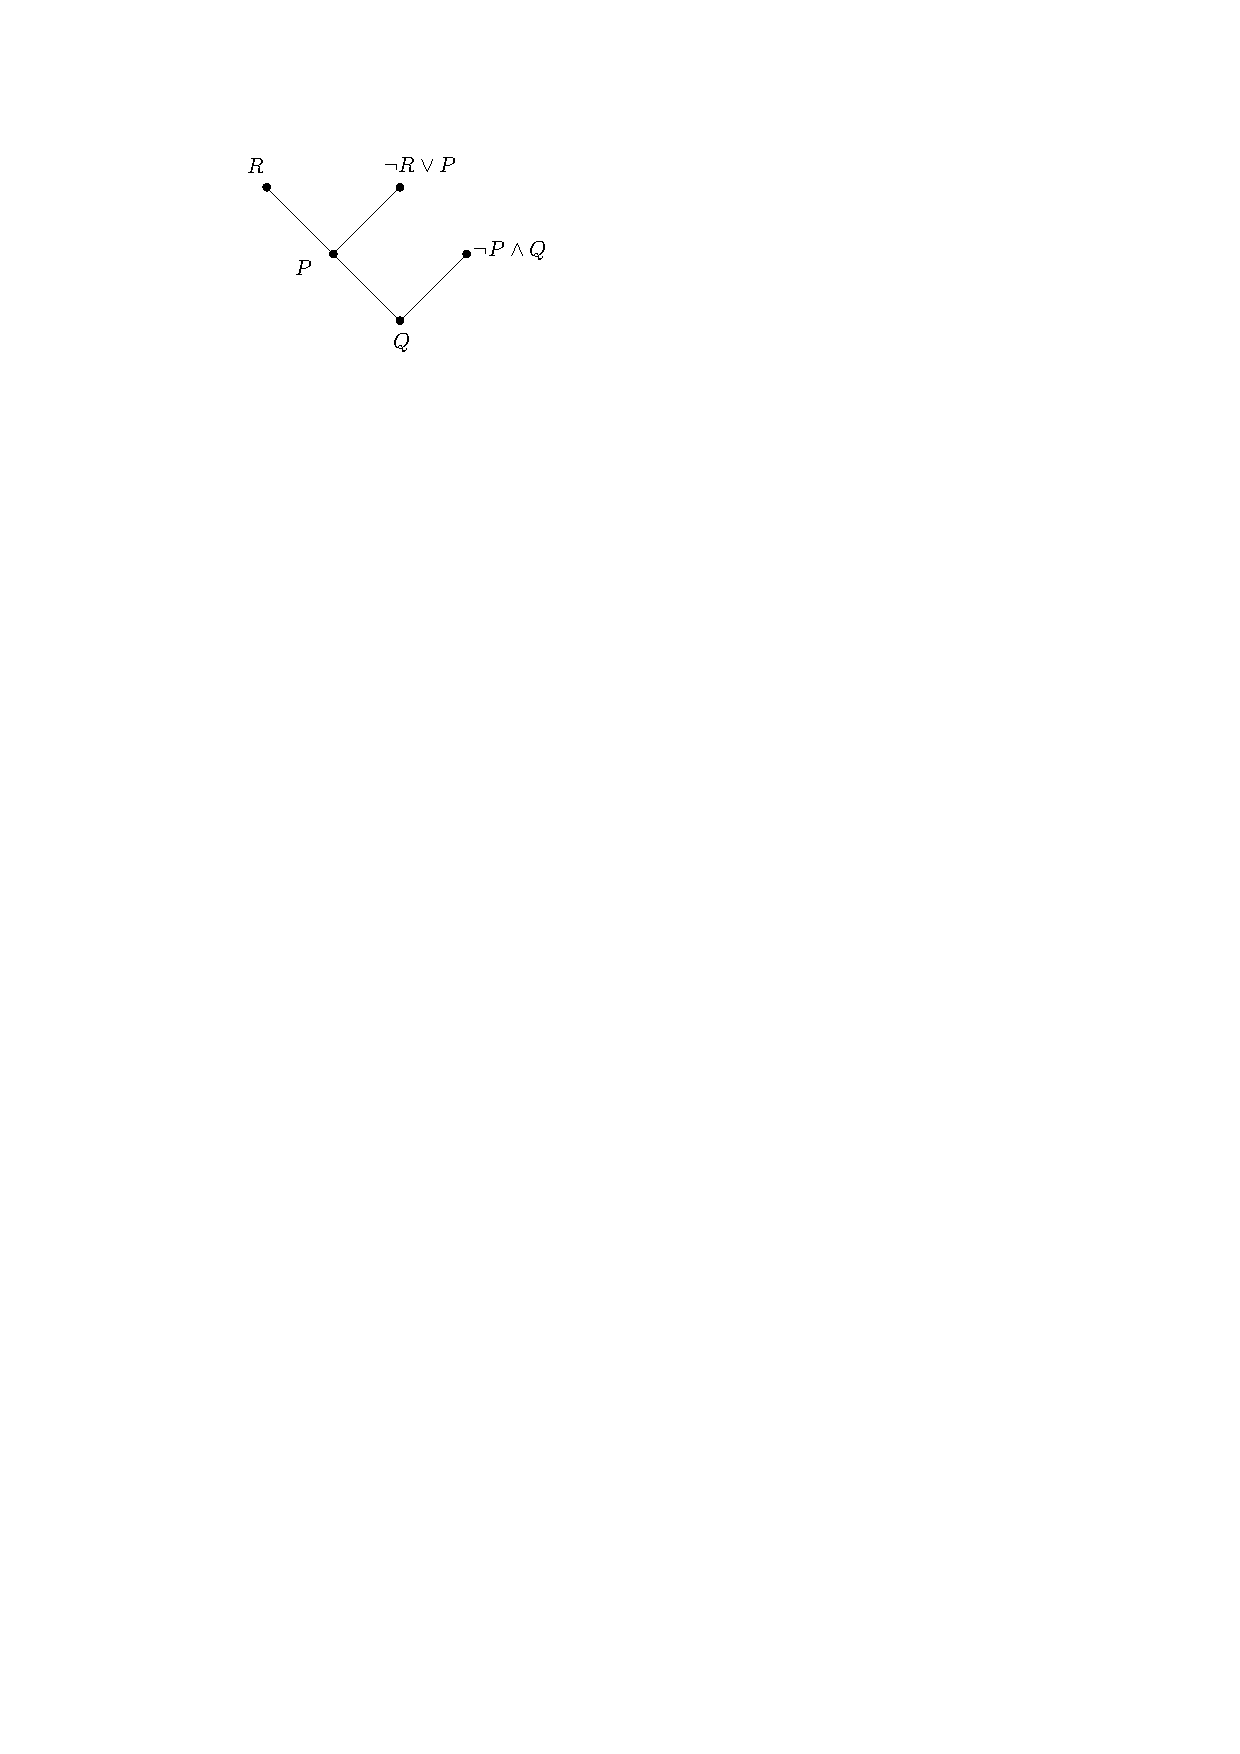
\includegraphics{image/标准-归结.pdf}
    \end{figure}
\end{example}

\begin{note}
    定理可拆分为包含条件和结论的蕴含式。
    \begin{itemize}
        \item \textcolor{main1}{如果满足“条件1”,“条件2”,$\dots$,“”,那么有“结论”}
        \item \textcolor{main1}{“条件1式”$\land$“条件2式”$\land\dots\land\dots\to$“结论式”}
    \end{itemize}
    定理证明就是要证明这个蕴含式是“永真式”
\end{note}
\begin{theorem}[基于归结的定理证明]
    证明以下:
    \begin{itemize}
        \item \textcolor{main1}{证明该式永真}:条件1式$\land$条件2式$\to$结论式
        \item \textcolor{main1}{证明该式永假}:$\lnot$(条件1式$\land$条件2式$\to$结论式)
        \item \textcolor{main1}{证明该式永假}:条件1式$\land$条件2式$\land\lnot$结论式
    \end{itemize}
\end{theorem}
\begin{note}
    归结为空意味着归结的子句间存在矛盾,推导出了永假的结果。即要证明这个式子永假,只要把这个式子归结出空就可以了。
\end{note}
\begin{example}
    机器人搬箱子,求证箱子超重。
    \begin{itemize}
        \item 机器人不能直接感知箱子是否超重
        \item 如果机器人电池有电并且箱子不超重,则机器人能够移动该箱子
        \item 已知电池有电且箱子搬不动
    \end{itemize}
    \begin{proof}
        有如下:
        设$A$:电池好、$B$:箱子超重、$C$:移动
        \begin{itemize}
            \item \textcolor{main1}{事实:}$A,\, \lnot C$
            \item \textcolor{main1}{定理:}$A\land \lnot B\to C$
            \item \textcolor{main1}{待证结论:}$B$
        \end{itemize}
        把\textcolor{main1}{所有条件和结论的非}写成合式公式,转化成标准子句:
        \[
            \begin{array}{l}
                A\land \lnot C\left( A\land \lnot B\to C \right)\land \lnot B\\
                =A\land \lnot C\left( \lnot A\lor B\lor C \right)\land \lnot B
            \end{array}
        \]        
        \begin{figure}[H]
            \centering
            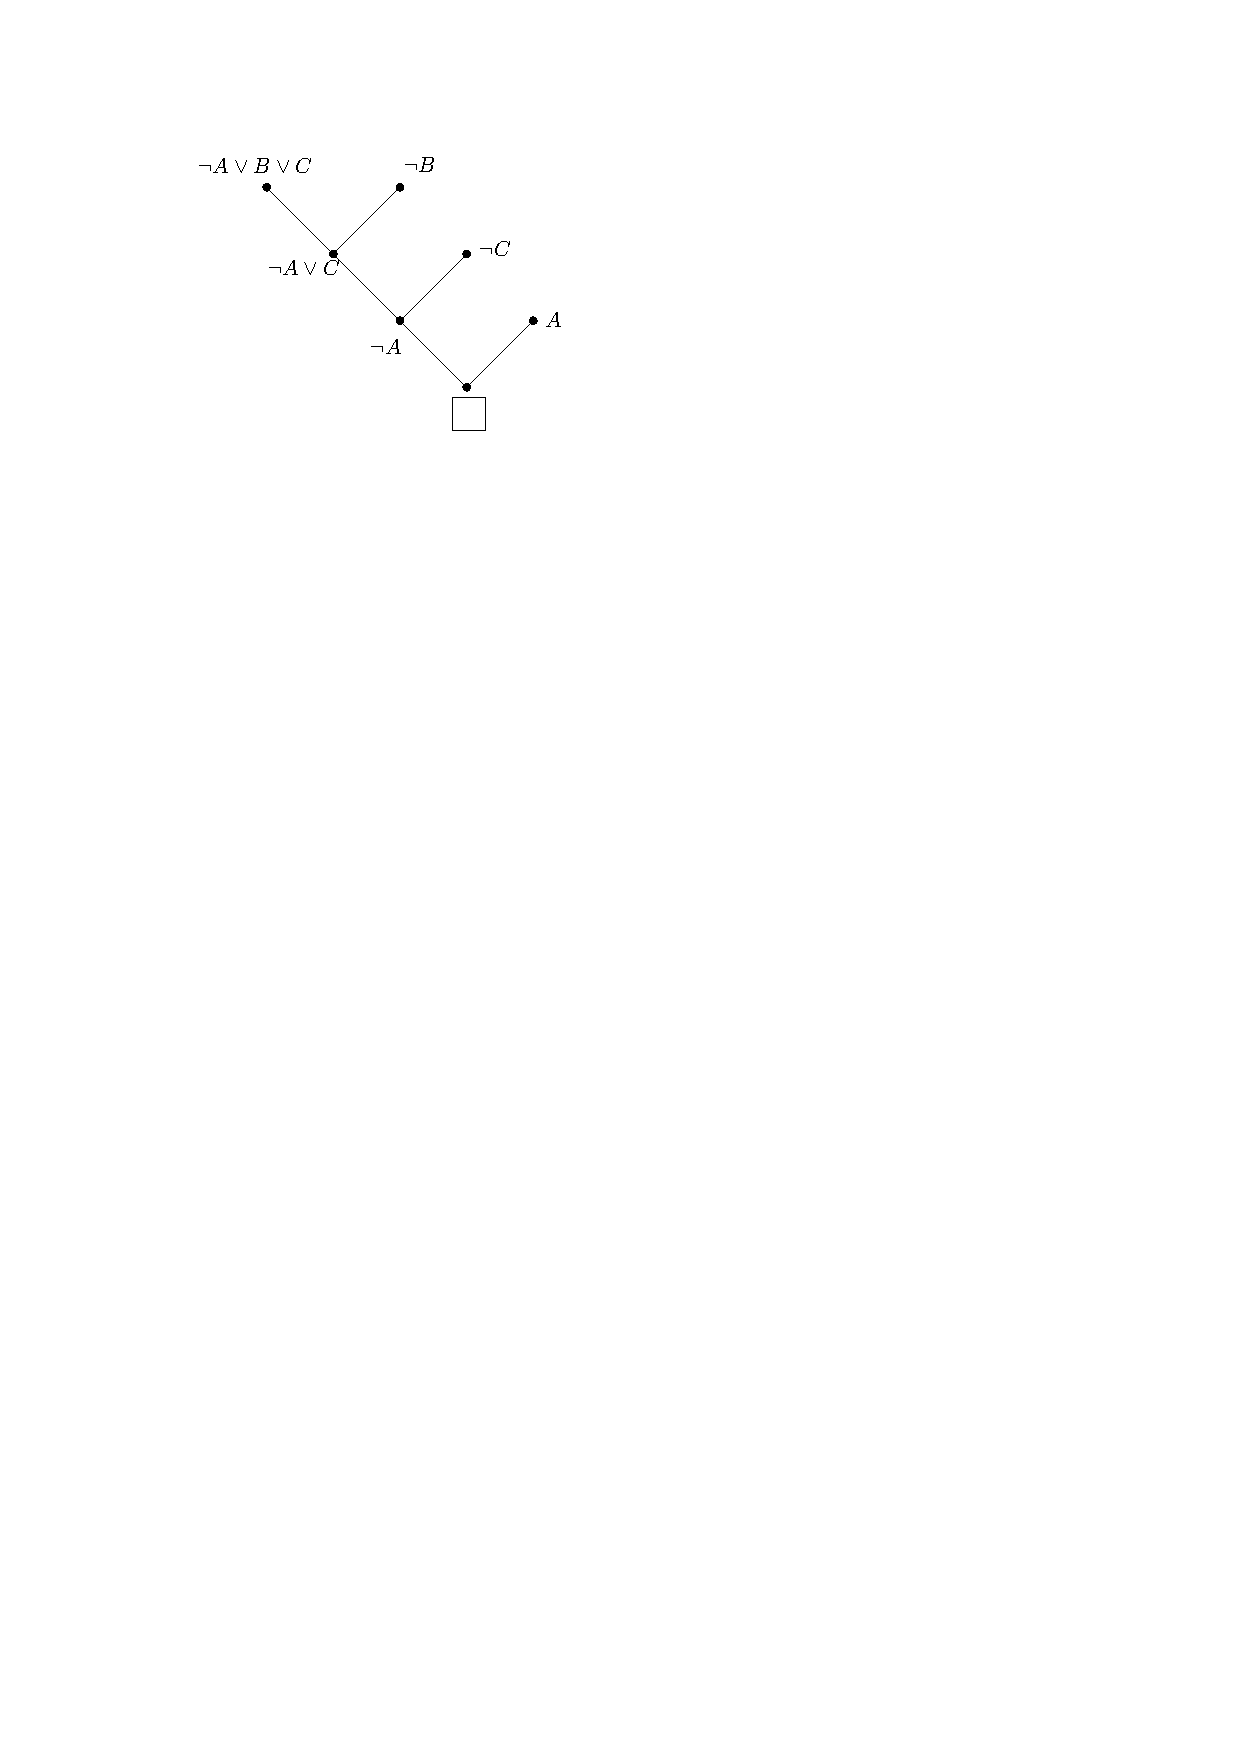
\includegraphics[width = .35\textwidth]{image/机器人搬箱子.pdf}
        \end{figure}
        证毕!
    \end{proof}
\end{example}
\begin{example}
    超级大间谍,谁是间谍?

    某个机密文件被泄露,保密局派出5个侦查员去调查
    \begin{itemize}
        \item 侦察员1说:“A与B中至少有一人作案”
        \item 侦察员2说:“B与C中至少有一人作案”;
        \item 侦察员3说:“C与D中至少有一人作案”;
        \item 侦察员4说:“A与C中至少有一人与此案无关”;
        \item 侦察员5说:“B与D中至少有一人与此案无关”。
    \end{itemize}
    证明:如果5个侦察员的话都可信,那么B和C都是间谍。
    \begin{proof}
        化为字句集合:C1:$A\lor B$、C2:$B\lor C$、C3:$C\lor D$、C4:$\lnot A \lor \lnot C$、C5:$\lnot B \lor \lnot D$、T1:$\lnot B\lor \lnot C$。把\textcolor{main1}{所有条件C1-C5和结论的非T1}写成合式公式
        \begin{figure}[H]
            \centering
            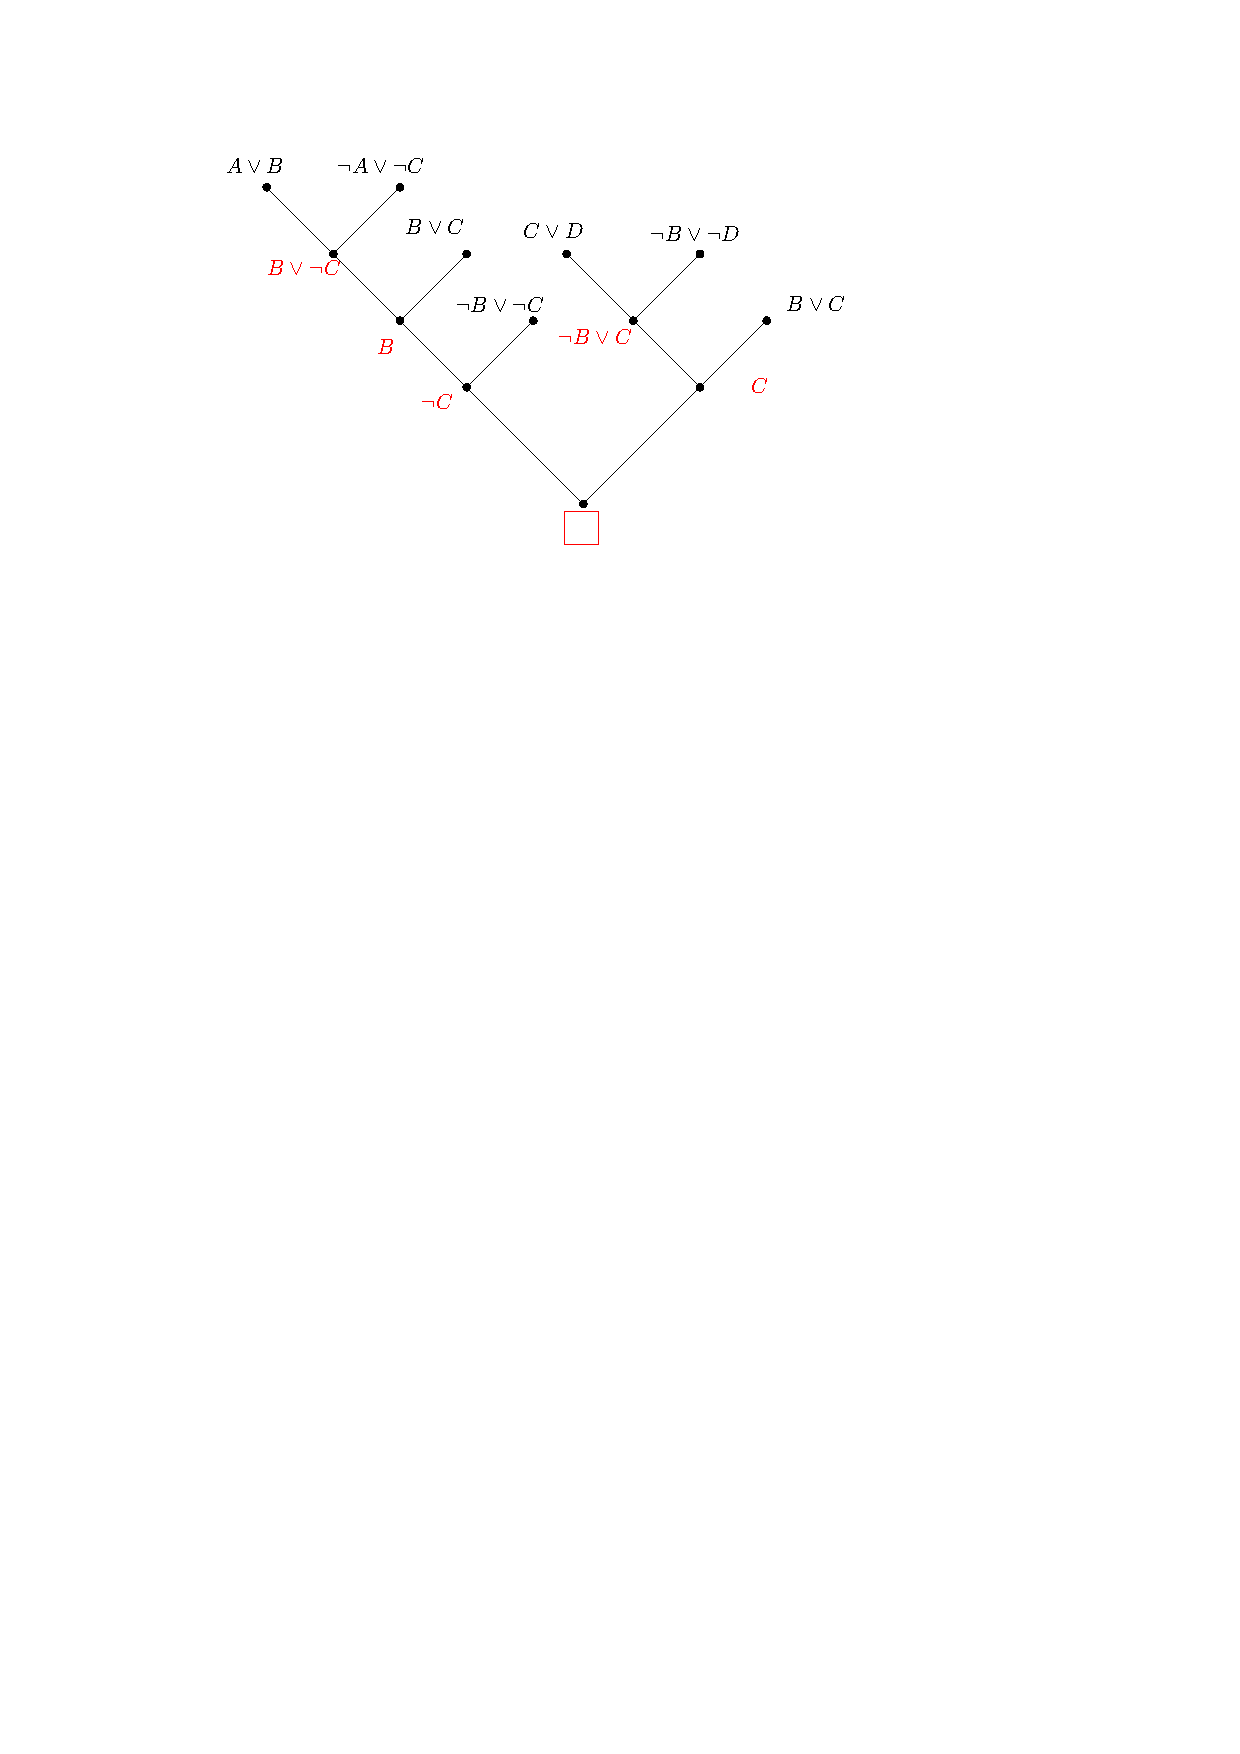
\includegraphics[width = .5\textwidth]{image/谁是间谍.pdf}
        \end{figure} 
        证毕!
    \end{proof}
\end{example}
采用归结原理进行命题逻辑定理证明的基本思想是
\begin{enumerate}[A]
    \item 归纳法
    \item 演绎法
    \item \textcolor{main1}{反证法}
    \item 枚举法
\end{enumerate}

\subsection{逻辑谓词}
\begin{note}
    命题逻辑的局限性:
    \begin{itemize}
        \item 不能表示事务的共同属性
        
        “亚里士多德是人,牛顿是人”需要用两个独立的命题来表示。这两个命题都是不可拆分的原子命题,两个命题共同的部分没法表示。
        \item 不能表达原子命题内部结构
        
        在这个原子命题中无法“张三和李四是同学”体现张三和李四的关系。
    \end{itemize}
\end{note}
\subsubsection{谓词逻辑的基本概念}
谓词逻辑由个体词、谓词、联结词及量词组成。
\begin{definition}[个体词(项)]
    指谓词描述的对象,能够独立存在的客体。

    \begin{itemize}
        \item \textcolor{main1}{常量:}张三、A、$\dots$,通常是对象的名字
        \item \textcolor{main1}{变量:}习惯上用小写字母表示,如x、 z等。Human(x)
        \item \textcolor{main1}{函数:}习惯上用小写字母或字母串表示,如$f,\,g$等。比如: father(小李)、LeftLeg (小李)、 sum(x,y)
    \end{itemize}
\end{definition}
\begin{definition}[谓词]
    用来刻画个体词的\textcolor{main1}{属性}或个体词之间的\textcolor{main1}{关系}
    
    \begin{itemize}
        \item 表示属性
        \item 表示关系
    \end{itemize}

    谓词不能单独使用,它必须与个体词结合才能构成谓词公式。
\end{definition}

\begin{definition}[联结词]
    表示谓词之间的关系
    \begin{itemize}
        \item 合取$\land$
        \item 析取$\land$
        \item 蕴含$\to$
        \item 非$\lnot$
    \end{itemize}
\end{definition}
\begin{definition}[量词]
    说明个体变量的取值范围。
    
    \begin{itemize}
        \item 全称量词,     
        表示“所有”,$\forall$
        \item 存在量词,        
        表示“存在”,$\exists$
    \end{itemize}
\end{definition}
\begin{note}
    使用量词应注意
    \begin{itemize}
        \item 一般情况下,$\to$是与$\forall$是一起的主要连接词
        \item 一般情况下,$\land$是与$\exists$是一起的主要连接词
    \end{itemize}
\end{note}
\begin{definition}[量词的辖域]
    \textcolor{main1}{量词的辖域}是邻接量词之后的最小子公式,\textcolor{main1}{因此除非辖域是个原子公式,否则应该在该子公式两端有括号}

    \begin{itemize}
        \item 例:$\forall x\, P(x)\to Q(x)$
        
        $\forall x$的辖域是$P(x)$
        \item 例:$\exists x\, (P(x)\to Q(x))\lor P(y,z)$
        
        $\exists x$的辖域是$P(x)\to Q(x)$
    \end{itemize}
\end{definition}
\begin{definition}[约束变元和自由变元]
    在一个量词的辖域中与该量词的\textcolor{main1}{指导变元}相同的变元称为\textcolor{main1}{约束变元},其他变元称为自由变元。

    例如:$\forall \textcolor{red}{x}\left( P(\textcolor{blue}{x})\lor Q(y) \right)\land (\exists \textcolor{red}{z})\left( R(\textcolor{blue}{z}) \right)$
\end{definition}
\begin{note}
    多个量词并用时

    $\forall x\exists yP(x,y)$与$\exists y\forall xP(x,y)$不等价

    $x,\,y$分别表示一个自然数;$P(x,y):,\,y>x$

    多个全称量词和存在量词混用时,顺序不可以颠倒。
\end{note}
\subsubsection{逻辑谓词的归结}
\begin{note}
    置换注意事项:

    \begin{itemize}
        \item 只有变量才能被置换,常量和函数不能被置换。
        \item 置换要整体进行,即不同位置的同一变量要一起置换。
        \item \textcolor{main1}{置换的变量不能出现在置换项中。} 即:对于置换$s = \left\{ t_1/x_1,t_2/x_2,\cdots,t_n/x_n \right\}$,任一变量$x_i$,不能出现在某个置换项$t_i$,中。
        \item 同一个变量不能被多个置换项同时置换。
        \item 置换不符合交换律:$s_1s_2\neq s_2s_1$
    \end{itemize}
\end{note}
\begin{note}
    置换与合一
    \begin{itemize}
        \item \textcolor{main1}{原始知识:}
        
        所有人都会死

        亚里士多德是人
        \item \textcolor{main1}{谓词公式:}
        
        \[
            \begin{array}{l}
                \forall x\,\left( Human(x)\to WillDie(x) \right)\\
                Human(Aristotle)
            \end{array}
        \]

        \item  \textcolor{main1}{化成子句:}
        
        \[
            \begin{array}{l}
                \lnot Human(x)\lor WillDie(x)\\
                Human(Aristotle)
            \end{array}
        \]
        这两个子句不能归结,因为形式上并不完全相同
        \item 用亚里士多德替换$x$,可以进行归结
        \item \textcolor{main1}{合一:}寻找项对变量的置换,以使两个合式公式表达一致。若存在一个置换$s$使得表达式集合$\{E_i\}$中每个元素经置换后有:$E_1s =E_2s = E_3s = \dots,$则称表达式集$\{E_i\}$是可合一的,这个置换$s$称为合一元。
        \item \textcolor{main1}{最一般合一元}$\sigma$(The most general unifier,mgu),$\left\{ w_i \right\}$的$\sigma$有如下特性

        如果$\theta$是$\left\{ w_i \right\}$任意合一元,那么存在一个置换$\lambda$使得$\left\{ w_i \right\}\theta = \left\{ w_i \right\}\sigma\lambda$,即$\sigma$是能够使合一的最小置换。
        \item 为何最需要最一般合一元
        
        求证:$\left\{ \lnot P(x,y)\lor \lnot Q(y,z), P(A,w) \right\}\Rightarrow \lnot Q(B,C)$
        \begin{figure}[htbp]
            \centering
            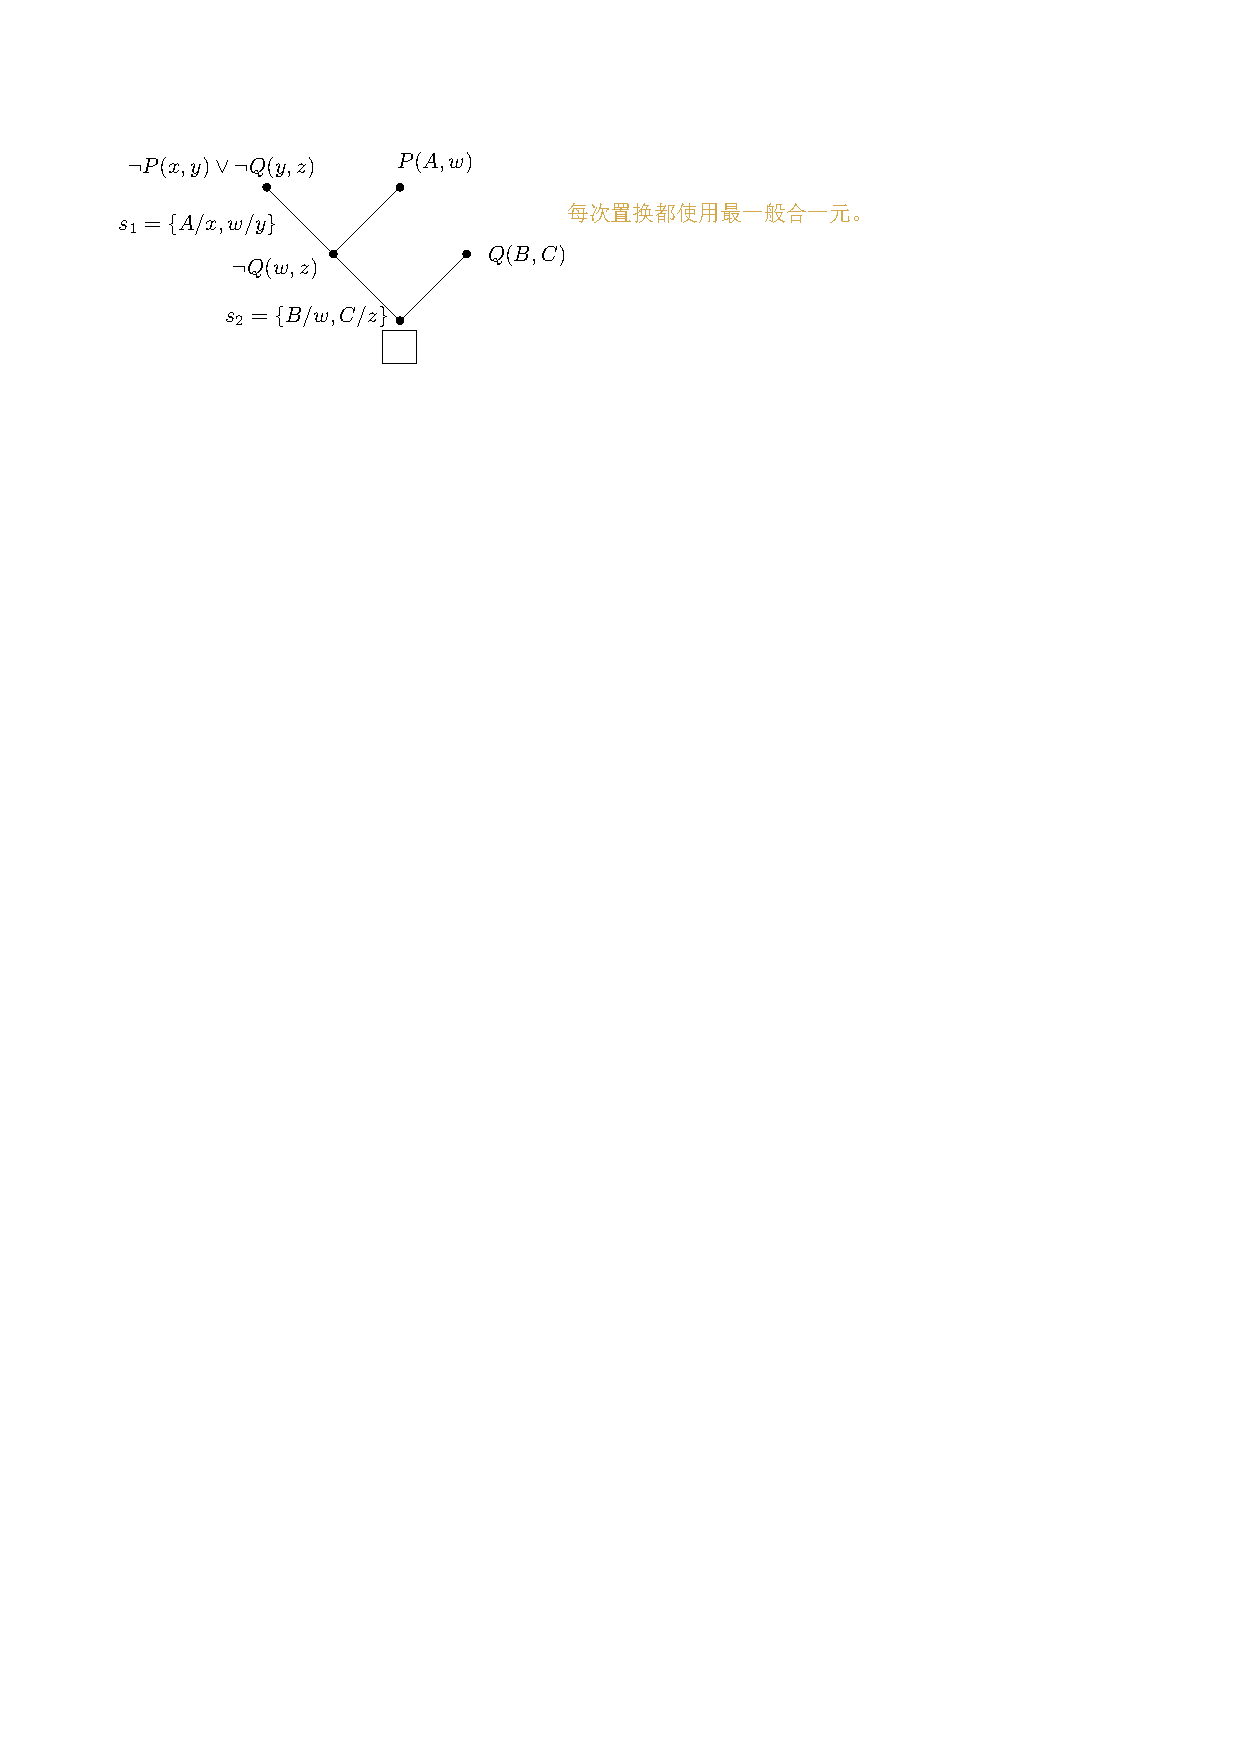
\includegraphics{image/最一般合一元.pdf}
        \end{figure}        
    \end{itemize}    
\end{note}
\begin{theorem}[归结原理]
    定理的证明过程:
    \begin{enumerate}
        \item 将\textcolor{main1}{结论的非}与\textcolor{main1}{所有条件式}进行合取,得到待证明的合式公式;
        \item 将上述合式公式化成可以归结的子句集形式;(\textcolor{main1}{子句间为合取关系,子句内为析取形式})
        \item 对上述式子进行归结,如果\textcolor{main1}{归结为空,则定理得证。}
    \end{enumerate}
\end{theorem}
\begin{note}
    命题演算中公式标准化过程:
    \begin{itemize}
        \item 消除蕴含符号
        
        使用蕴含表达式$P\to Q\equiv \lnot P\land Q$
        \item 否定深入
        
        减少否定符号的范围,否定符号$\lnot$最多只用到一个命题符号上
        \item 转换成子句的合区范式
        
        字句内析取、子句间合区
        \item 形成子句合集
    \end{itemize}
\end{note}
\begin{note}
    谓词公式化为标准子句:

    目的:将谓词公式化为\textcolor{main1}{机器可以接收、处理}的标准形式,这种标准形式是\textcolor{main1}{不含量词的子句集}
    相比命题公式标准化的难点:
    \begin{itemize}
        \item 全称量词和存在量词处理
        \item 各种变量名称如何处理
    \end{itemize}

    \textcolor{main1}{标准化步骤}:
    \begin{enumerate}
        \item 消去蕴含符号
        \item 否定深入(减少否定符号的范围)
        \item \textcolor{main1}{变量标准化(每个量词有唯一的变量符号)}
        
        \textcolor{main1}{例如:}
        \begin{itemize}
            \item 量词辖域不重叠
            
            $\left( \forall x \right)P(x)\lor \left( \forall x \right)Q(x)$转化为$\left( \forall x \right)P(x)\lor \left( \forall \textcolor{main1}{y} \right)Q(\textcolor{main1}{y})$
            \item 量词辖域重叠
            
            $\left( \forall x \right)\left( P(x)\to \left( \exists x \right)Q(x) \right)$转化为$\left( \forall x \right)\left( P(x)\to \left( \exists \textcolor{main1}{y} \right)Q(\textcolor{main1}{y}) \right)$
        \end{itemize}
        通过改变变量名称,使每个量词修饰的变量有自己唯一的变量名。(\textcolor{main1}{不同量词修饰的变量符号不同})
        \item \textcolor{main1}{消去存在量词}
        
        \begin{itemize}
            \item 如果存在量词不受全称量词修饰:直接例化即可
            
            $\exists xP(x)$实例化为$P(A)$,要求$A$必须是新的常量符号
            \item 如果存在量词受全称量词修饰:使用Skolem函数
            
            $\left( \forall x \right)\left( \left( \exists y \right)\operatorname{Cap}(x,y) \right)$,用$g(x)$替换$y$,消去存在量词得到$\left( \forall x \right)\operatorname{Cap}(x,g(x))$,Skolem函数必须是新的
        \end{itemize}

        消去存在量词,\textcolor{main1}{存在量词}的\textcolor{main1}{约束变元}使用关于\textcolor{main1}{全称量词}的\textcolor{main1}{指导变元的函数}来代替

        如果存在量词处在多个全称量词的辖域内,则同时受多个全称量词共同影响,Skolem函数为关于多个全称量词修饰变量的函数。
        \item \textcolor{main1}{消去全称量词}
        \begin{itemize}
            \item 直接将全称量词的符号去除。
            \item 经过前面几步,已经不存在量词修饰的变量,剩下的变量可以任意取值,所以没必要保留全称量词符号。
        \end{itemize}

        \item 把公式化为合取范式(子句间为合取关系,子句内为析取形式)写成子句形式(消除合取符号)
        \item \textcolor{main1}{更换变量名称(一个变量符号不用于多个子句)}
        
        更换变量符号的名称,使一个变量符号不出现在一个以上的子句中。

        对于子句集
        \[
            \begin{array}{l}
                \{ \lnot P(x_1)\lor \lnot P(y)\lor P(f(x_1,y)),\\
                    \lnot P(x_2)\lor Q(x_2,g(x_2))\\
                    \lnot P(x_3)\lor \lnot P(g(x_3))\}
            \end{array}
        \]
    \end{enumerate}
\end{note}
\begin{example}
    将下列谓词公式化为标准子式
    \begin{itemize}
        \item $\forall x\left( \left( \forall y P(x,y) \right) \to \lnot \left( \forall y\left( Q(x,y)\to R(x,y) \right) \right) \right)$
        \begin{enumerate}
            \item 消去蕴含符号
            \[
                \forall x\left(\lnot \left( \forall y P(x,y) \right) \lor \lnot \left( \forall y\left( \lnot Q(x,y)\lor R(x,y) \right) \right) \right)
            \]
            \item 否定深入
            \[
                \forall x\left(\exists y \lnot P(x,y)  \lor \left( \exists y\left( Q(x,y)\land \lnot R(x,y) \right) \right) \right)            
            \]
            \item 变量标准化
            \[
                \forall x\left(\exists y \lnot P(x,y)  \lor \left( \exists z\left( Q(x,z)\land \lnot R(x,z) \right) \right) \right)
            \]
            \item 消去存在量词
            \[
                \forall x\left(\lnot P(x,f(x))  \lor \left( Q(x,g(x))\land \lnot R(x,g(x)) \right) \right)
            \]
            \item 消去全称量词
            \[
                \lnot P(x,f(x))  \lor \left( Q(x,g(x))\land \lnot R(x,g(x)) \right)
            \]
            \item 化为合取范式 
            \[
                \left( \lnot P(x,f(x)) \lor Q(x,g(x)) \right) \land  \left(\lnot P(x,f(x)) \lnot R(x,g(x)) \right)
            \]
            \item 化为子句集形式
            \[
                \begin{array}{l}
                    \{  \lnot P(x,f(x)) \lor Q(x,g(x)),\\ 
                    \lnot P(x,f(x)) \lnot R(x,g(x)) \}
                \end{array}
            \]
            \item 更换变量名称
            \[
                \begin{array}{l}
                    \{  \lnot P(x,f(x)) \lor Q(x,g(x)),\\ 
                    \lnot P(y,f(y)) \lnot R(y,g(y)) \}
                \end{array}
            \]
        \end{enumerate}
        \item $\left( (\exists x)P(x)\lor (\exists x)Q(x) \right)\to \left( (\exists x)(P(x)\lor Q(x)) \right)$
        \begin{enumerate}
            \item 消去蕴含符号
            \[
                \lnot \left( (\exists x)P(x)\lor (\exists x)Q(x) \right)\lor \left( (\exists x)(P(x)\lor Q(x)) \right)
            \]
            \item 否定深入
            \[
                \left((\forall x)\lnot P(x)\land (\forall  x)\lnot Q(x) \right)\lor \left( (\exists x)(P(x)\lor Q(x)) \right) 
            \]
            \item 变量标准化
            \[
                \left((\forall x)\lnot P(x)\land (\forall  y)\lnot Q(y) \right)\lor \left( (\exists z)(P(z)\lor Q(z)) \right) 
            \]
            \item 消去存在量词
            \[
                \left((\forall x)\lnot P(x)\land (\forall  y)\lnot Q(y) \right)\lor \left( P(A)\lor Q(A)\right) 
            \]
            \item 消去全称量词
            \[
                \left(\lnot P(x)\land \lnot Q(y) \right)\lor \left( P(A)\lor Q(A)\right) 
            \]
            \item 化为合取范式
            \[
                \left(\lnot P(x)\lor P(A)\lor Q(A) \right)\land \left(\lnot Q(y)\lor P(A)\lor Q(A) \right)
            \]
            \item 化为子句集形式
            \[
                \begin{array}{l}
                    \{  \lnot P(x)\lor P(A)\lor Q(A),\\ 
                    \lnot Q(y)\lor P(A)\lor Q(A) \}
                \end{array}
            \]
            \item 更换变量名称
            \[
                \begin{array}{l}
                    \{  \lnot P(x)\lor P(A)\lor Q(A),\\ 
                    \lnot Q(y)\lor P(A)\lor Q(A) \}
                \end{array}
            \]
        \end{enumerate}
    \end{itemize}
\end{example}
\subsubsection{定理证明和求解}
\begin{note}
    谓词定理自动归结证明过程
    \begin{itemize}
        \item 将合式公式化为子句集的过程不同
        
        因为谓词逻辑引入了个体词和量词,所以化为子句时和命题化为子句的步骤是不一样的
        \item 归结过程不同
        
        因为个体词有变量和常量,所以谓词归结的过程和命题归结相比需要置换和合一。
    \end{itemize}
\end{note}
\begin{example}
    机器人搬箱子的归结证明

    已知:27号房间的所有箱子都比29号房间的箱子小。现在机器人知道箱子A在27号或29号房间中,箱子B在27号房间中,且B不比A小。\textcolor{main1}{试证明箱子A在27号房间中}
    \begin{proof}
        有以下谓词公式
        \begin{itemize}
            \item F1:\,$ \forall x\forall y\left( P(x)\land P(y)\land Inroom(x,27)\land Inroom(y,29)\to Smaller(x,y)  \right) $
            \item F2:\,$ Inroom(A,27)\lor Inroom(A,29) $
            \item F3:\,$ Inroom(B,27)\land \lnot Smaller(B,A) $
            \item F4:\,$P(A)$
            \item F5:\,$P(B)$
            \item T:\,$ \lnot Inroom(A,27) $
        \end{itemize}    
        化为子句集形式
        \begin{itemize}
            \item C1:\,$ \lnot P(x)\lor \lnot P(y)\lor \lnot Inroom(x,27)\lor\lnot Inroom(y,29)\lor Smaller(x,y)  $
            \item C2\,:$ Inroom(A,27)\lor Inroom(A,29) $
            \item C3\,:$ Inroom(B,27) $
            \item C4\,:$ \lnot Smaller(B,A) $
            \item C5\,:$P(A)$
            \item C6\,:$P(B)$
            \item C7\,:$ \lnot Inroom(A,27) $
        \end{itemize}
        \textcolor{main1}{归结定理证明}
        \begin{figure}[htbp]
            \centering
            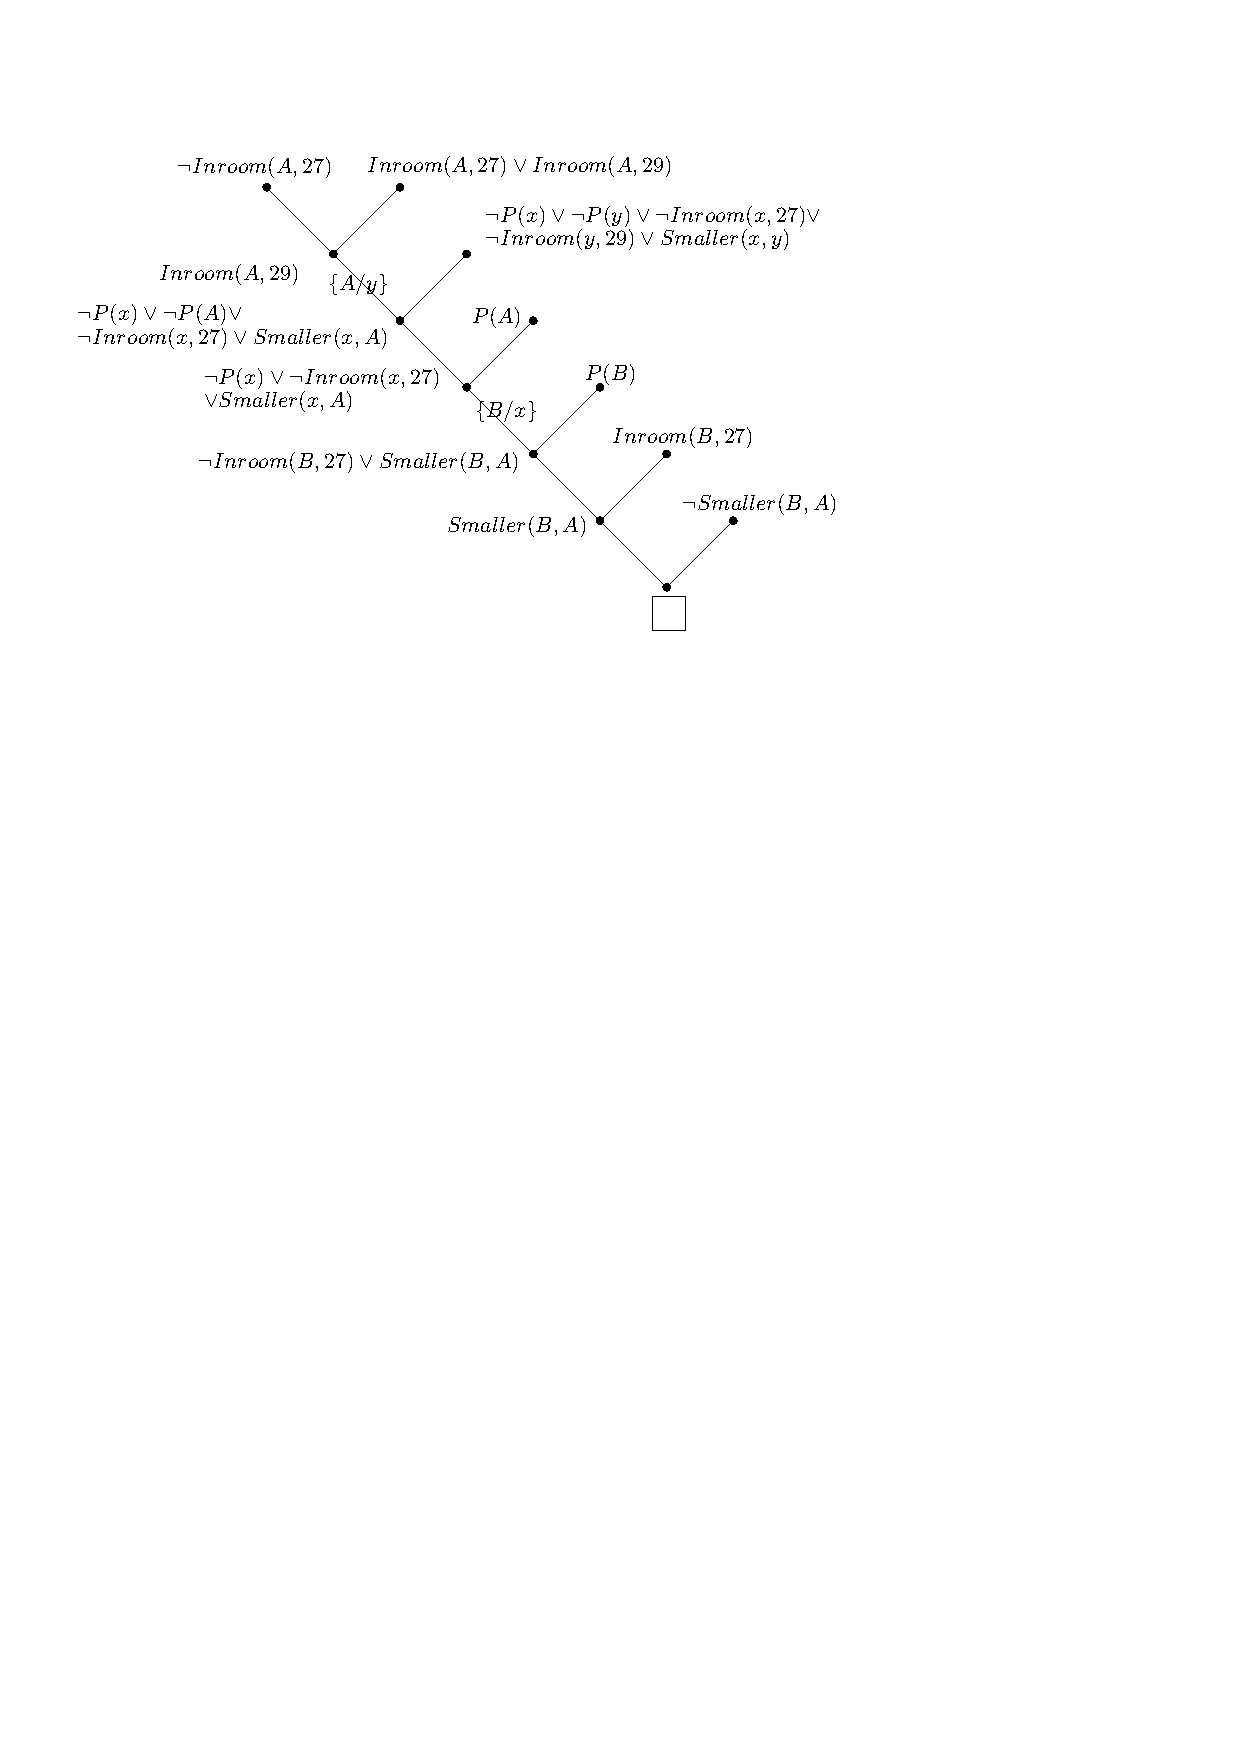
\includegraphics{image/定理证明例子.pdf}
        \end{figure}
    \end{proof}
\end{example}

\begin{example}
    机器人搬箱子的问题求解

    已知:27号房间的所有箱子都比29号房间的箱子小。现在机器人知道箱子A在27号或29号房间中,箱子B在27号房间中,且B不比A小。\textcolor{main1}{问箱子A在哪个房间?}

    \textcolor{main1}{解:}有以下谓词公式
    \begin{itemize}
        \item F1:\,$ \forall x\forall y\left( P(x)\land P(y)\land Inroom(x,27)\land Inroom(y,27)\to Smaller(x,y)  \right) $
        \item F2:\,$ Inroom(A,27)\lor Inroom(A,29) $
        \item F3:\,$ Inroom(B,27)\land \lnot Smaller(B,A) $
        \item F4:\,$P(A)$
        \item F5:\,$P(B)$
        \item T:\,$ \left( \exists u \right)\,Inroom(A,u) $
    \end{itemize}    
    化为子句集形式
    \begin{itemize}
        \item C1:\,$ \lnot P(x)\lor \lnot P(y)\lor \lnot Inroom(x,27)\lor\lnot Inroom(y,27)\lor Smaller(x,y)  $
        \item C2\,:$ Inroom(A,27)\lor Inroom(A,29) $
        \item C3\,:$ Inroom(B,27) $
        \item C4\,:$ \lnot Smaller(B,A) $
        \item C5\,:$P(A)$
        \item C6\,:$P(B)$
        \item C7\,:$ \lnot Inroom(A,u) $
    \end{itemize}
    \begin{figure}[htbp]
        \centering
        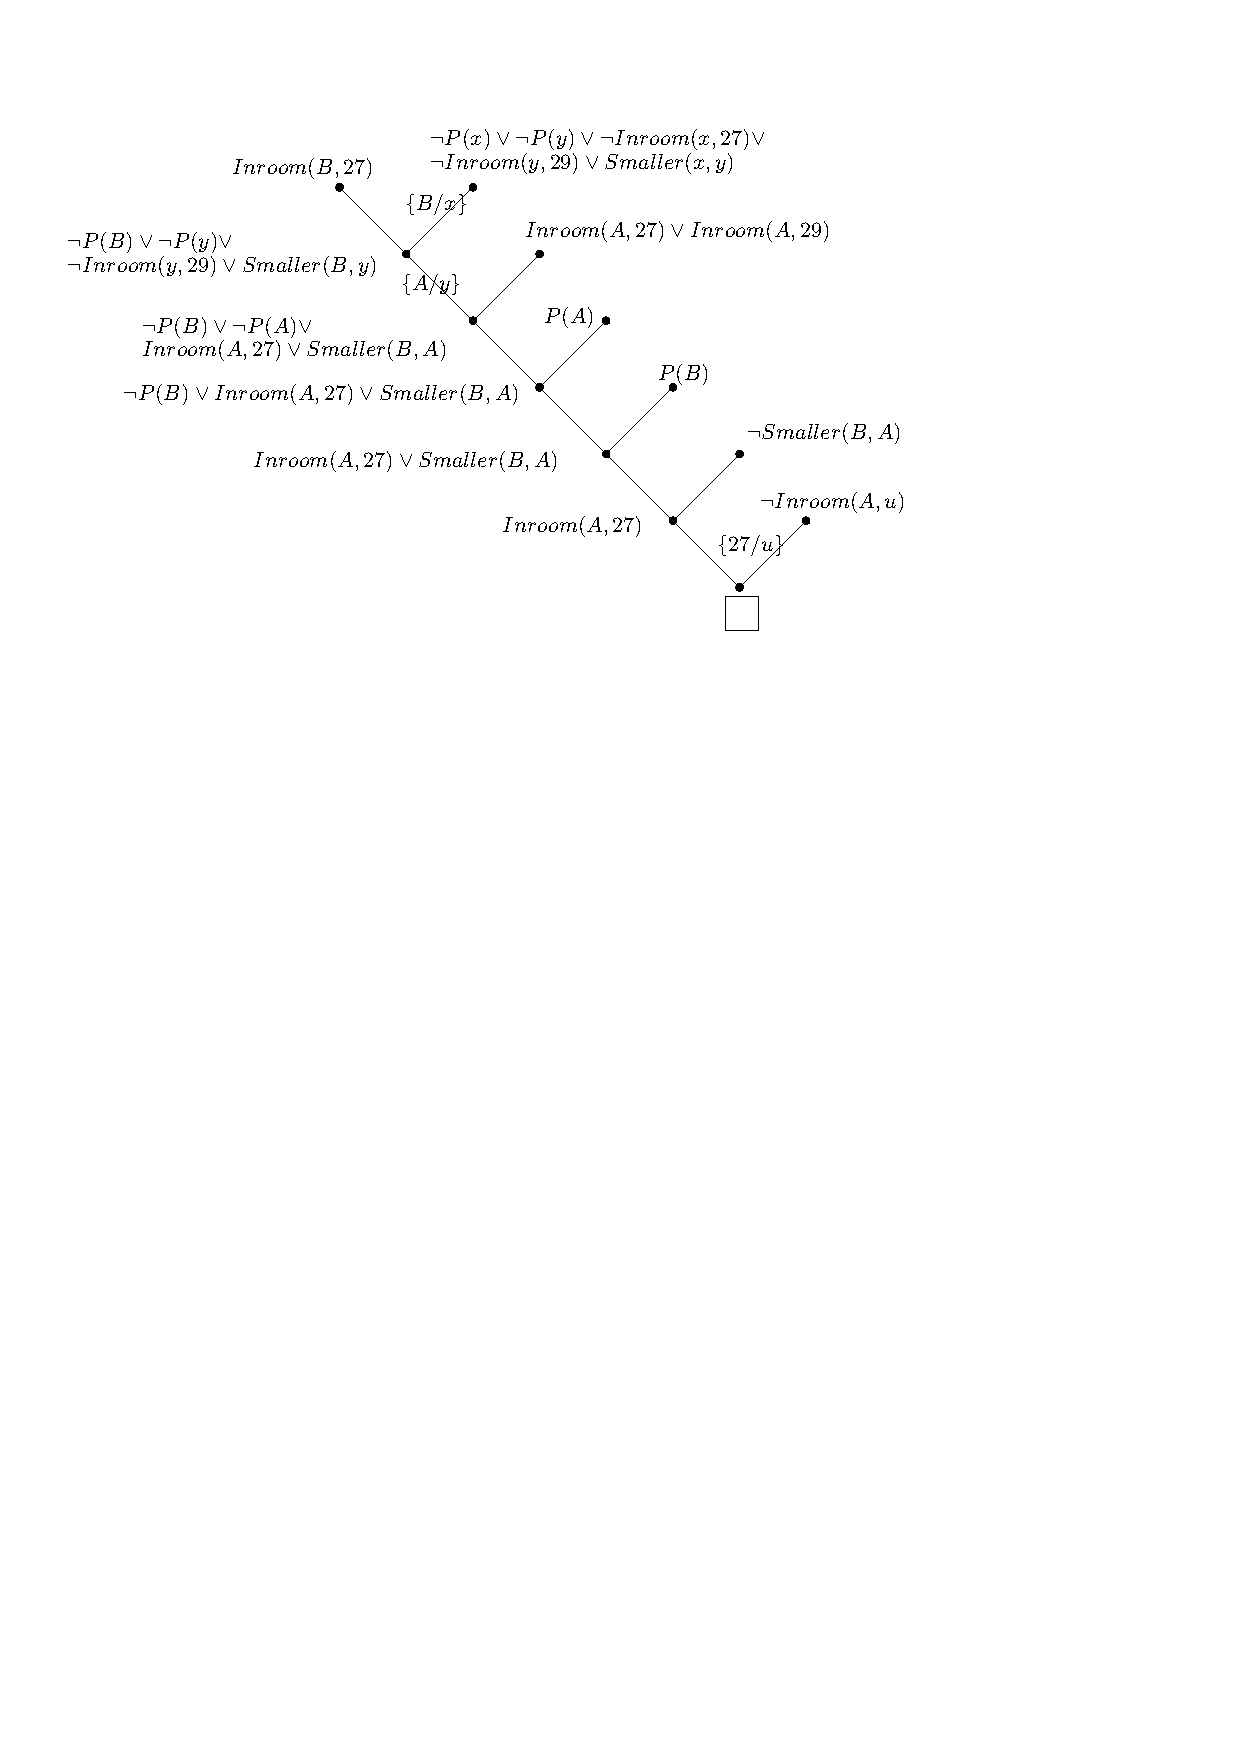
\includegraphics[width = .7\textwidth]{image/问题求解例子.pdf}
    \end{figure}

    用归结来回答由合式公式表示的关于领域知识的问题,而不只是证明一个定理。例如,不仅要证明形如$(\exists u)W(u)$的定理,而且想得到已经证明存在的$u$。
    为此,将文字$Ans(u)$加到要证明定理的否定子句中,执行归结直到只剩下一个回答文字。\textcolor{main1}{加入子句$\lnot W(u)\lor Ans(u)$}
    \begin{figure}[htbp]
        \centering
        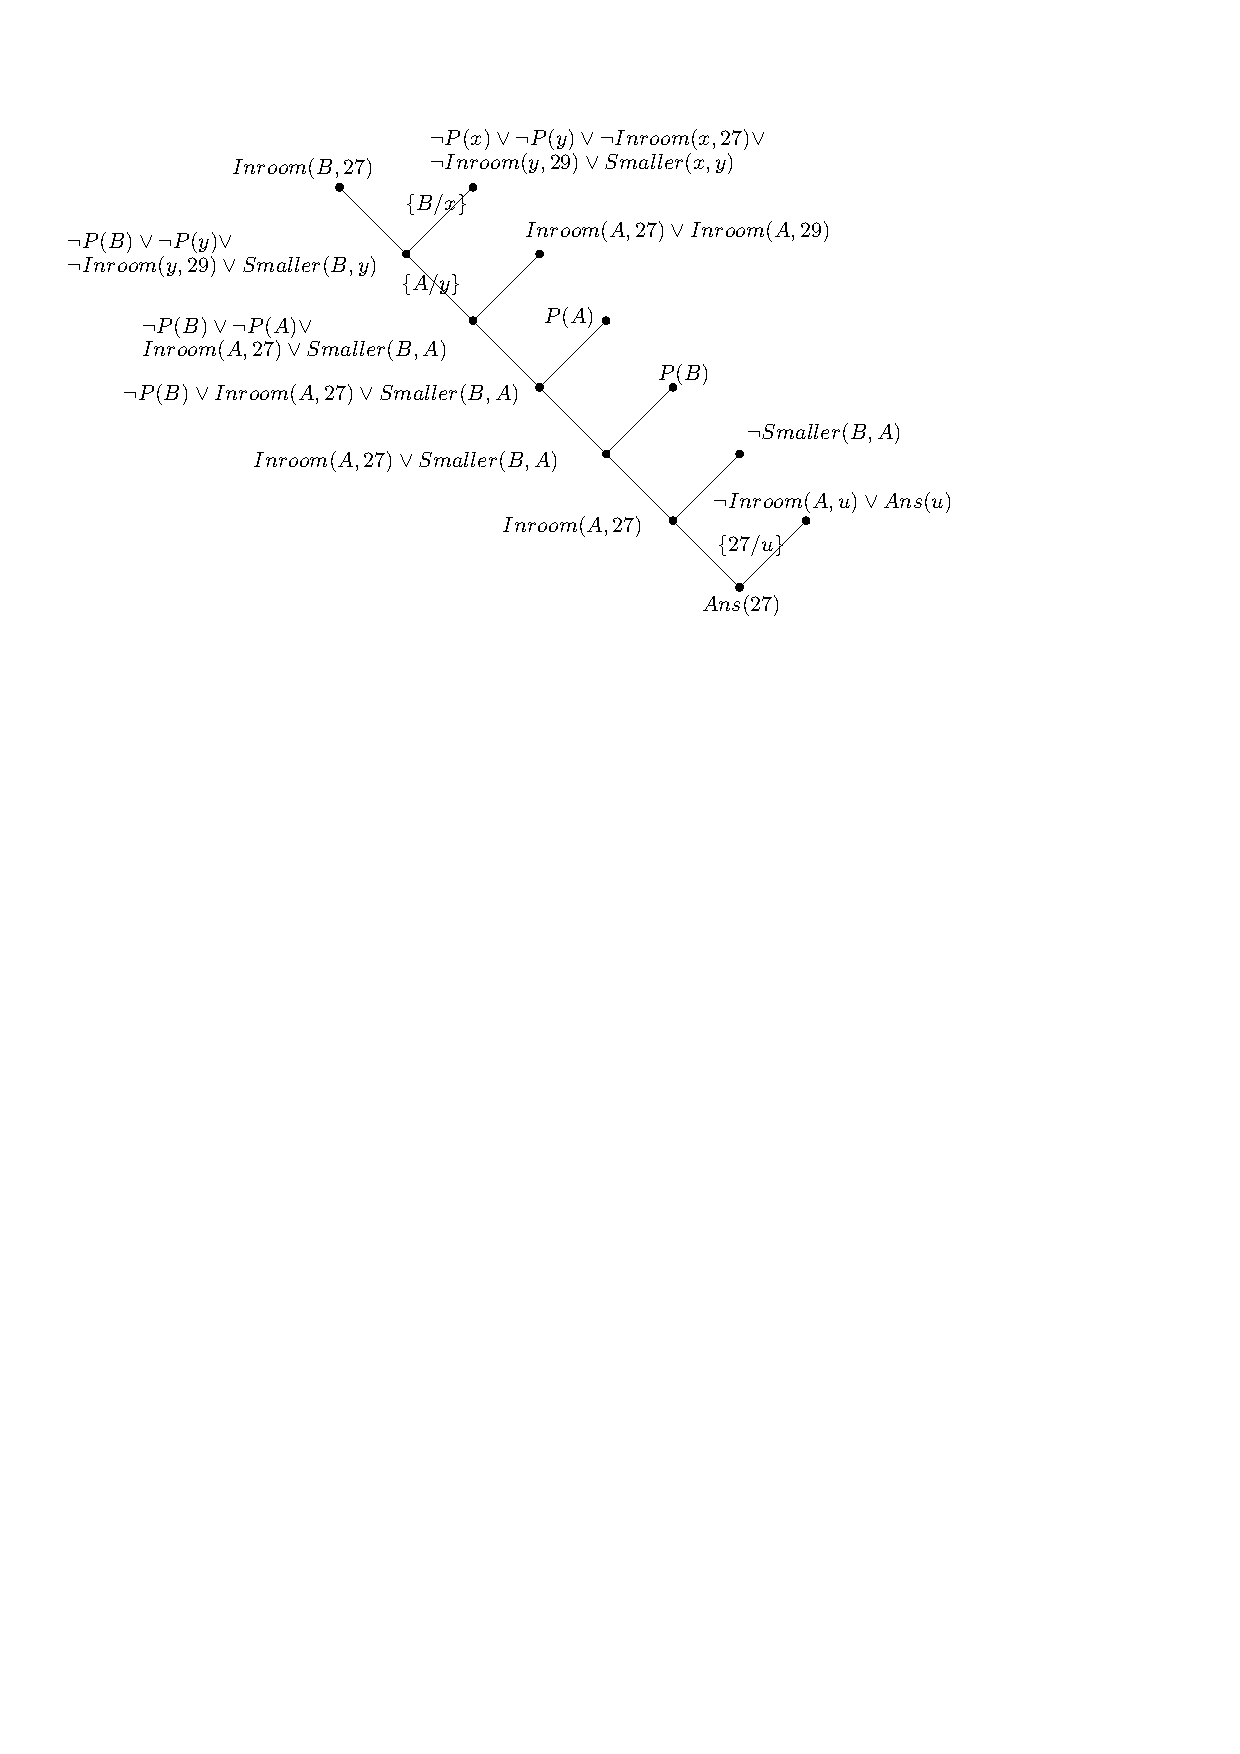
\includegraphics[width = .7\textwidth]{image/问题求解例子+Ans.pdf}
    \end{figure}
\end{example}

\subsection{不确定知识与推理}
\subsubsection{不确定性描述}
\begin{figure}[htbp]
    \centering
    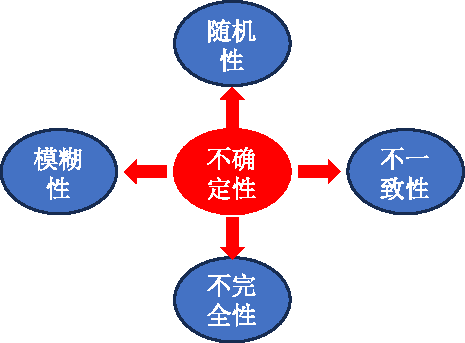
\includegraphics[scale = 0.7]{image/不确定性.pdf}
\end{figure}
\begin{itemize}
    \item 随机性
    
    如果乌云密布并且电闪雷鸣,则很可能要下暴雨。
    
    如果头痛发烧,则大概是患了感冒。
    \item 模糊性
    
    姚明是个高个子。
    
    张三和李四是好朋友。
    \item 不完全性
    
    战场上,交战双方对对手的信息掌握往往是不完全的。
    
    警方破案过程中,所掌握的关于罪犯的有关信息,往往就是不完全的。
    \item 不一致性
    
    牛顿运动定律对于宏观世界是正确的,但对于微观世界和宇观世界却是不适合的。
\end{itemize}
\subsubsection{不确定领域的知识表示}
\begin{example}
    例医疗诊断中,医生知道脑膜炎会引起病人脖子僵硬(如70\%的概率)﹔此外,医生还了解一些无条件事实:病人患脑膜炎先验概率1/50000,而任何一个病人脖子僵硬的先验概率为1\%。目前有一病人脖子僵硬,判断是否为脑膜炎。

    令$s$表示“病人脖子僵硬”,$m$表示“病人患有脑膜炎”,则有
    \[
        \begin{array}{l}
            p(s|m) = 0.7\\
            p(m) = 1/50000\\
            p(s) = 0.01\\
            p(m|s) = \dfrac{p(s|m)p(m)}{p(s)} = \dfrac{0.7\times 1/50000}{0.01} = 0.0014
        \end{array}
    \]
\end{example}
\subsubsection{贝叶斯网络}
\begin{definition}[条件概率表(CPT)]
    对于一个变量$Z$,CPT定义了一个条件分布$P(Z|parent(Z))$;其中,$parent(Z)$表示$Z$的父节点。

    \begin{itemize}
        \item 如果结点$X$没有父结点,则表中只包含先验概率$P(X)$;
        \item 如果结点$X$只有一个父结点$Y$,则表中包含条件概率$P(X| Y)$;
        \item 如果结点$X$有多个父结点$\{Y_1,Y_2,\cdots,Y_k\}$,则表中包含条件概率$P(X|Y_1,Y_2,\cdots,Y_k)$。
    \end{itemize}
    \begin{figure}[htbp]
        \centering
        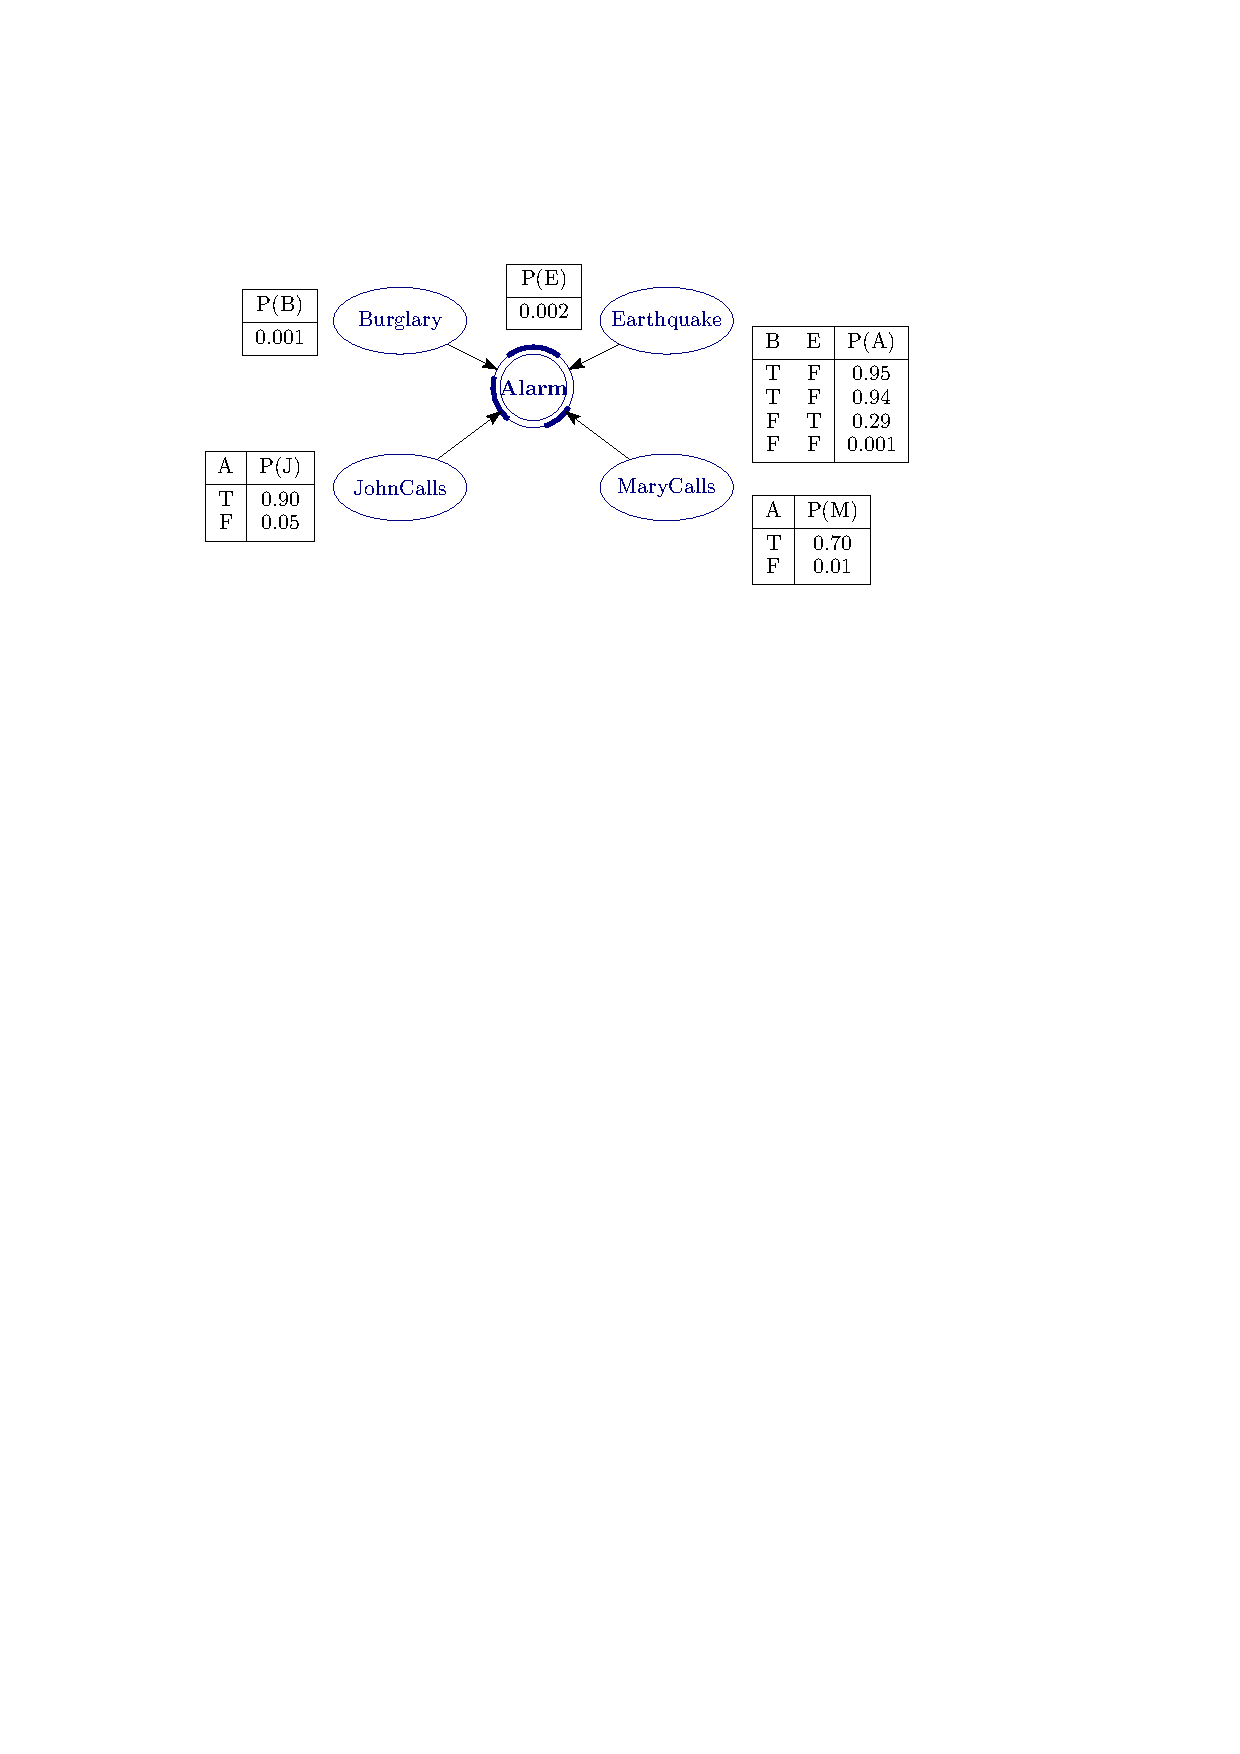
\includegraphics{image/CPT.pdf}
    \end{figure}
    在\textcolor{blue}{非因果方向}上,确定条件独立是困难的,且网络的压缩效果也不理想。
\end{definition}
\begin{note}
    贝叶斯网络(Bayesian Networks, BN)语法语义
    \begin{itemize}
        \item 全局语义:全联合概率分布与局部条件概率分布之间的关系
        \begin{figure}[htbp]
            \centering
            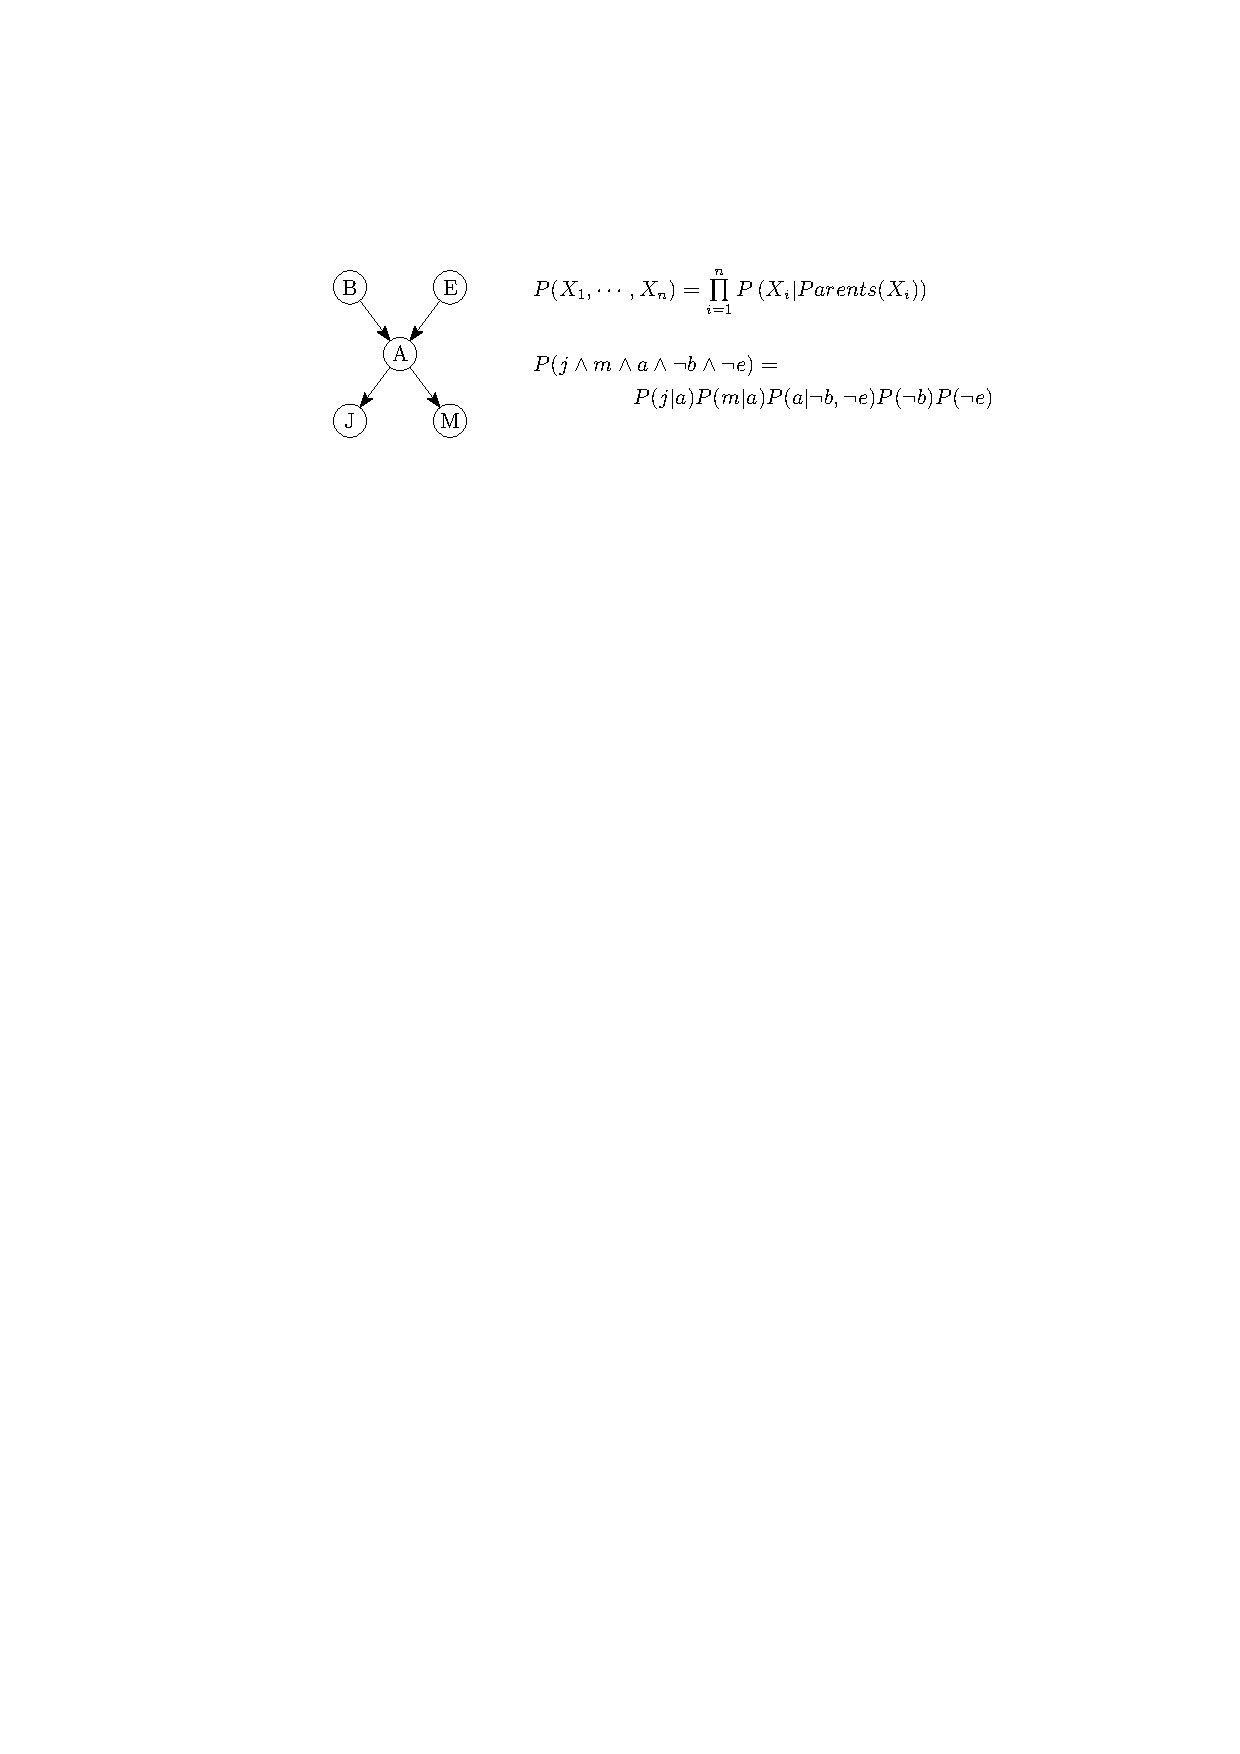
\includegraphics{image/贝叶斯网络全局语法语义.pdf}
        \end{figure}
        \item 局部语义:充分利用条件独立性,分析哪些变量之间是独立的
        
        贝叶斯网络的一个结点,如果它的父结点已知,则该结点条件独立于它的所有非后代结点
        \begin{figure}[htbp]
            \centering
            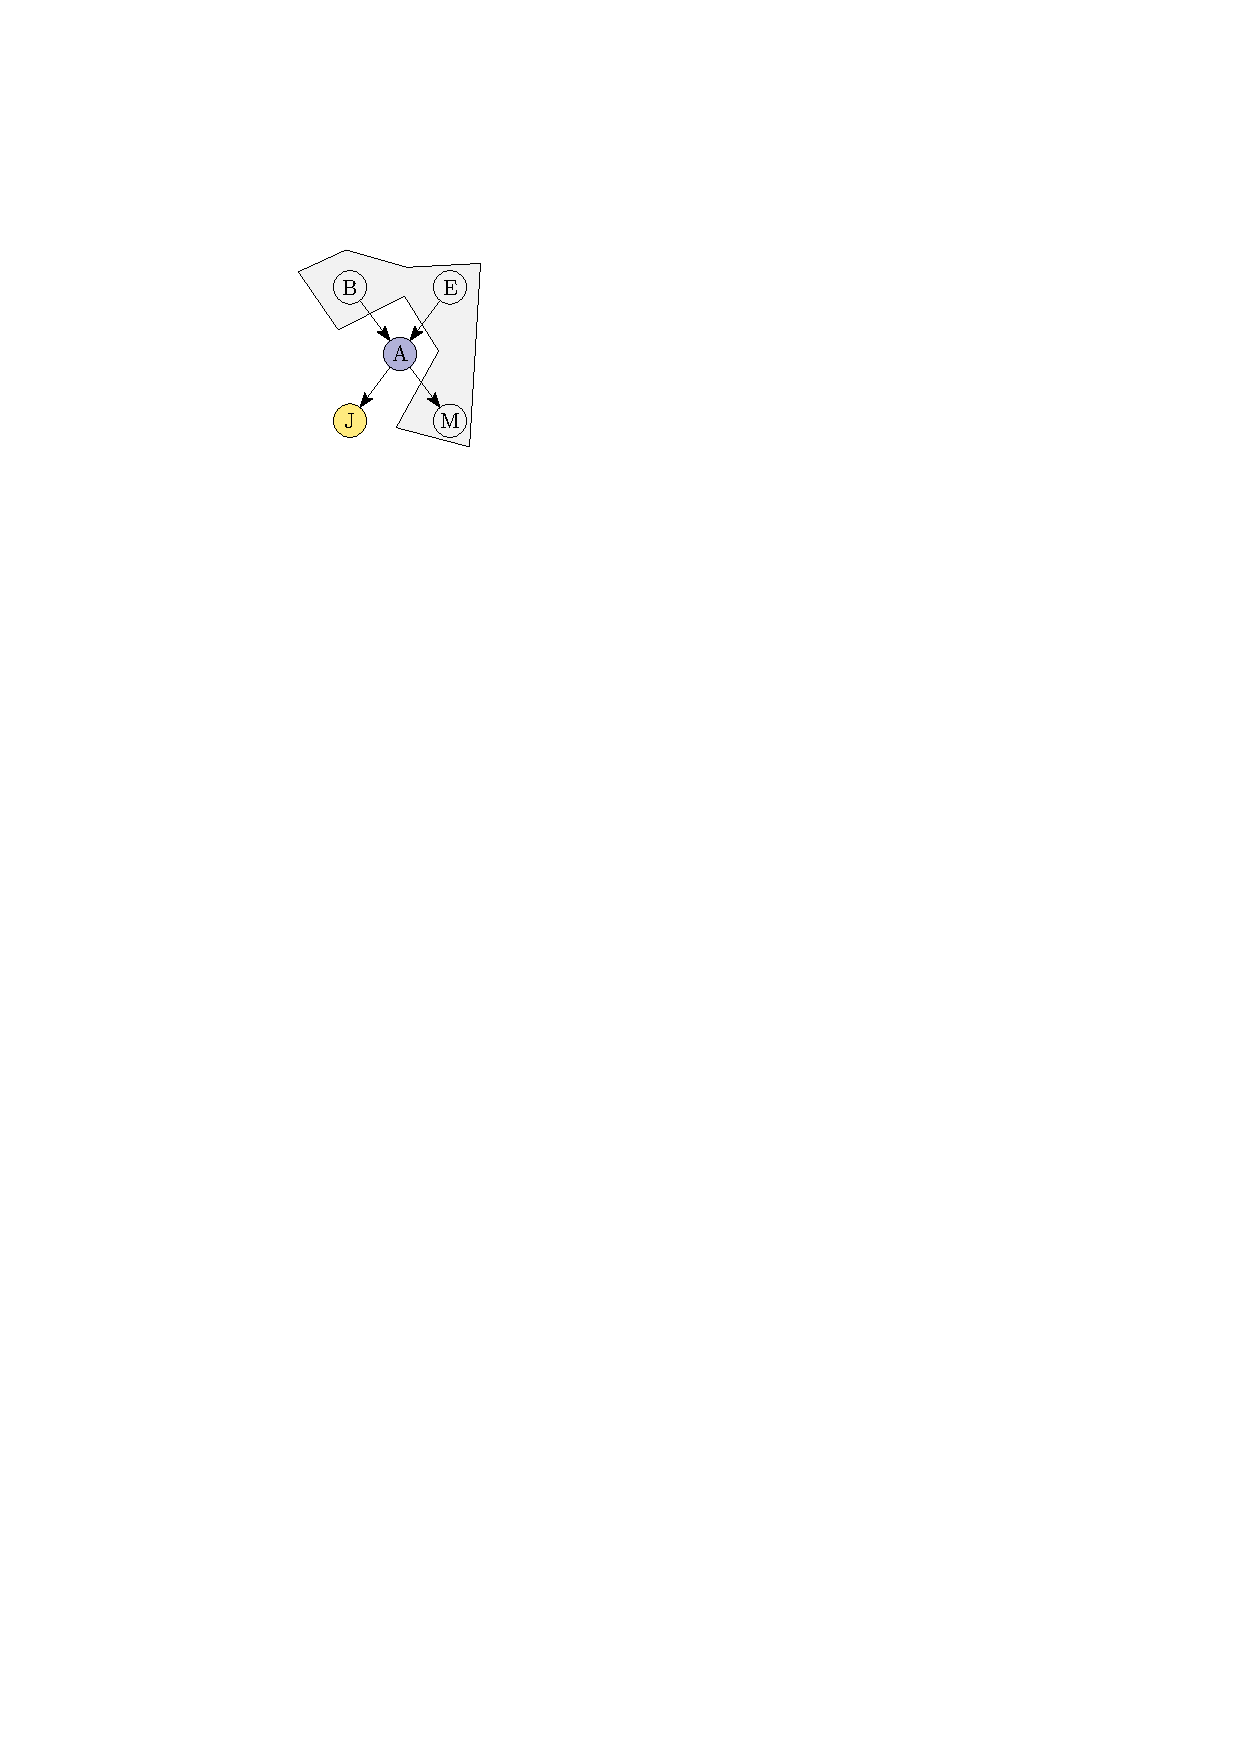
\includegraphics{image/贝叶斯网络局部语法语义.pdf}
        \end{figure}
    \end{itemize}
\end{note}
\begin{example}
    构造贝叶斯网络的步骤,主要包括:
    \begin{enumerate}[A]
        \item \textcolor{main1}{确定变量集和变量域}
        \item \textcolor{main1}{确定网络结构}
        \item \textcolor{main1}{确定节点条件概率表}
        \item 确定网络的规模
    \end{enumerate}
\end{example}
\subsubsection{基于贝叶斯网络的推理}
\begin{example}
    考虑下图所示的贝叶斯网络,解答下列问题:
    \begin{figure}[htbp]
        \centering
        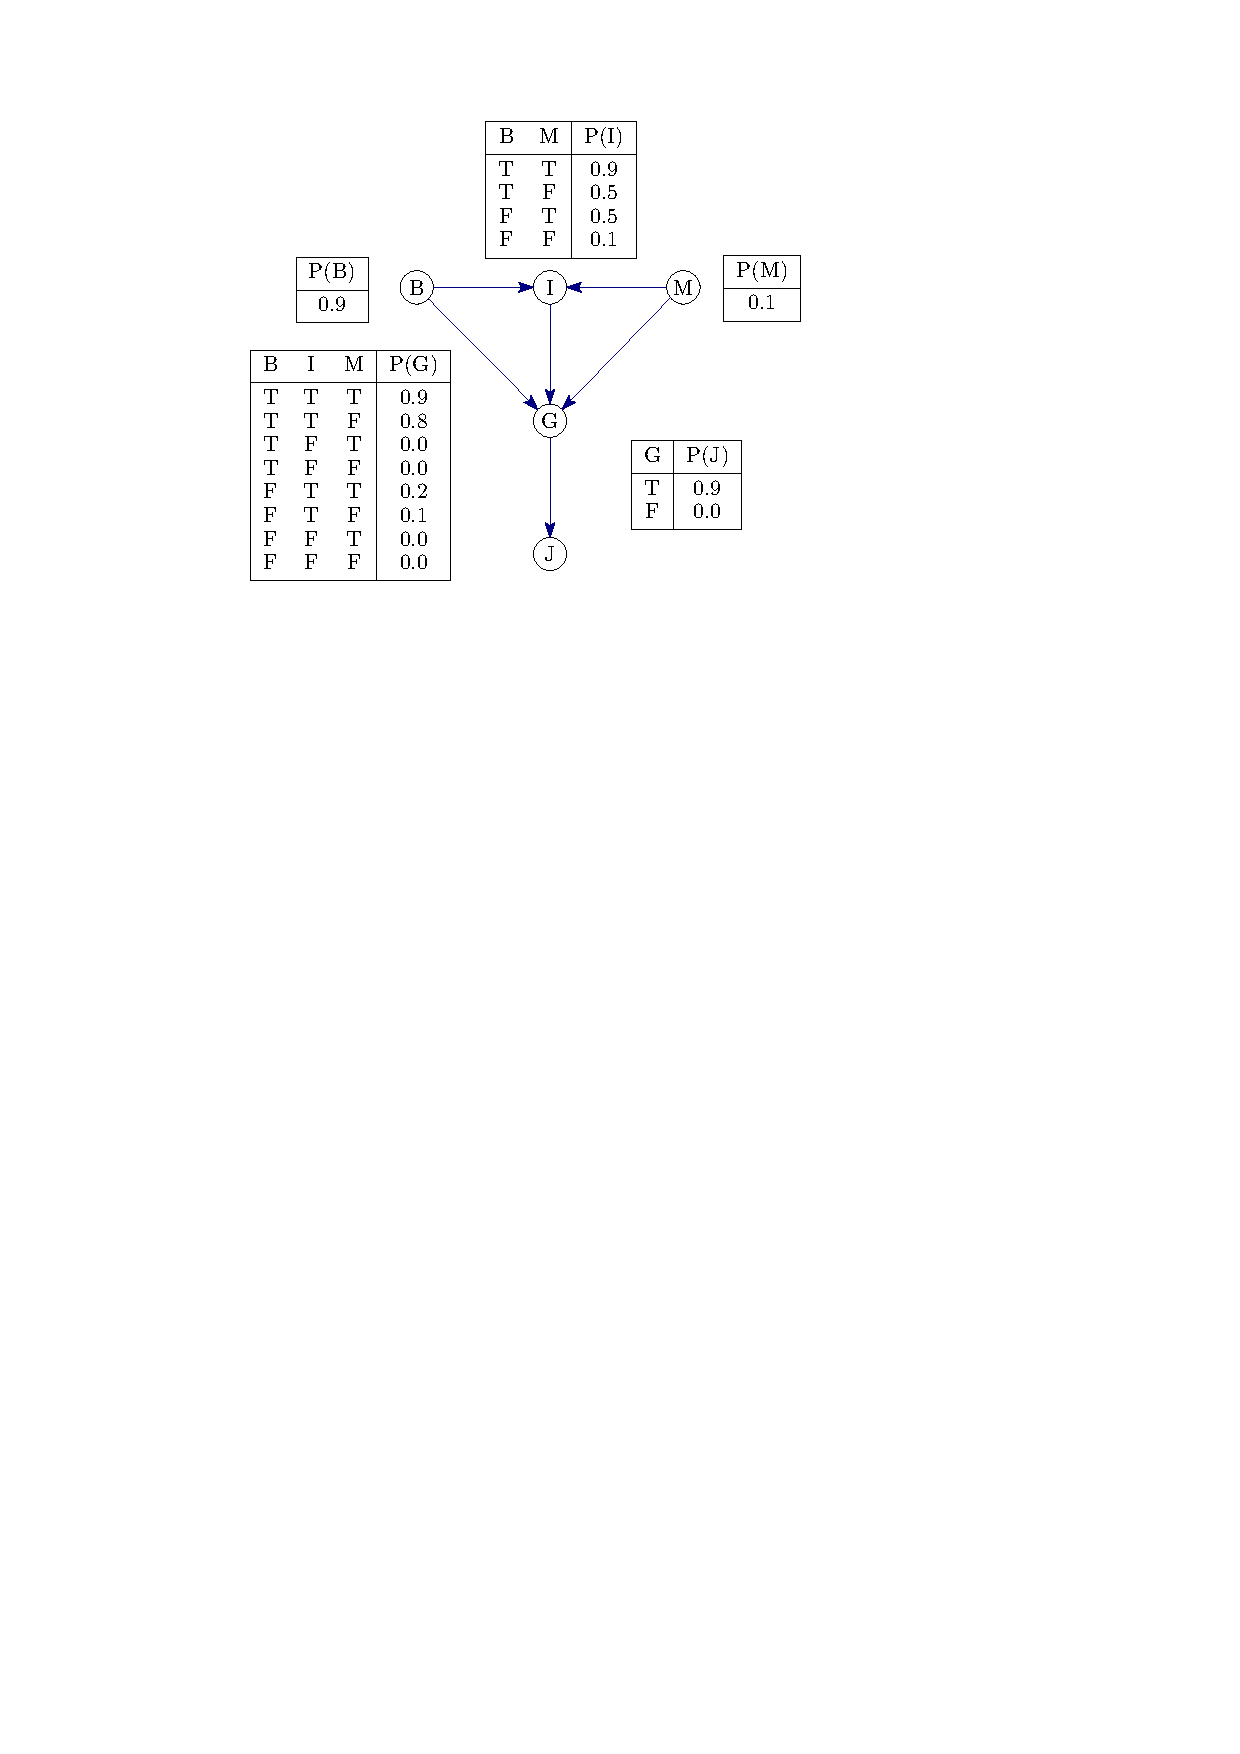
\includegraphics[scale = 0.8]{image/贝叶斯网络.pdf}
    \end{figure}
    \begin{enumerate}
        \item 网路结构能否断言下列语句?若不能,请写出正确表达式
        \begin{enumerate}
            \item $P(B,I,M) = P(B)P(I)P(M)$
            
            不能,正确表达式为$P(B,I,M) = P(I|B,M)P(B)P(M)$
            \item $P(J|G) = P(J|G,I)$
            
            能
            \item $P(M|G,B,I) = P(M|G,B,I,J)$
            
            能
        \end{enumerate}
        \item 计算$P(b,i,\lnot m,G,\lnot j)$
        \[
            \begin{array}{ll}
                &P(b,i,\lnot m,g,\lnot j) = P(\lnot j|g)P(g|b,i,\lnot m)P(i|b,\lnot m)P(b)P(\lnot m)\\
                &=(1-0.9)\times 0.8\times 0.5\times 0.9\times (1-0.1)\\
                &=0.0324
            \end{array}
        \]

        \[
            \begin{array}{ll}
                &P(b,i,\lnot m,\lnot g,\lnot j) = P(\lnot j|\lnot g)P(\lnot g|b,i,\lnot m)P(i|b,\lnot m)P(b)P(\lnot m)\\
                &=(1-0)\times (1-0.8)\times 0.5\times 0.9\times (1-0.1)\\
                &=0.081
            \end{array}
        \]
        另一种写法
        \[
            P(b,i,\lnot m,G,\lnot j) = \langle 0.0324,0.081 \rangle
        \]
    \end{enumerate}
\end{example}
